\chapter{JWAT - Workload Analyzer Tool}
\label{cha:usrman} A computer system can be viewed as a set of
hardware and software resources that are used in a time-variant
fashion by the processing requests generated by the user. During
any given time interval, the users submit their processing
requests to the systems by inputting sets of programs, data,
commands, requests for web sites or file downloads, etc. All this
input requests are usually designated by the collective term of
$workload$. Every time the value of a system or network
performance index is given, the workload under which that values
obtained must be reported or, at any rate, known, since
performance cannot be expressed by quantities independent of the
system's workload. Thus, no evaluation problem can be adequately
solved if the workloads to be processed by the systems or
transmitted over a network are not specified.\\
The quantitative description of a workload's characteristics is
commonly called {\it workload characterization}. A
characterization is usually done in terms of workload parameters
that can affect system behavior and are defined in a form suitable
for a desired use. Thus, a workload is characterized correctly if,
and only if, its result is a set of quantitative parameters
selected according to the goals of the characterization operation.
Workload characterization is fundamentally important in all
performance evaluation studies and is indispensable for designing
useful workload models.\\
A workload may be regarded as a set of vectors in a space with a
number of dimensions equal to the number of the workload
parameters used to describe each element considered. Since the
amount of resulting data is generally considerable, their analysis
for the purpose of identifying groups of components with similar
characteristics will have to be performed by statistical
techniques that can handle multidimensional samples, that is,
techniques that deal with multiple factors.

The JWAT tool is based on the application of a set of statistical
techniques oriented towards the characterization of log data
representing resource utilizations, traffic of requests, user web
paths, etc. Its application provides the input data for the models
to be used in all types of performance evaluation studies.

The main window of  JWAT (\autoref{fig:jwat_start_screen}) is
opened pressing the

\includegraphics[scale=.15]{img/jwat/Manual/JWATIcon.eps} button
in the JMT suite main window.
\begin{figure}[htbp]
    \begin{center}
        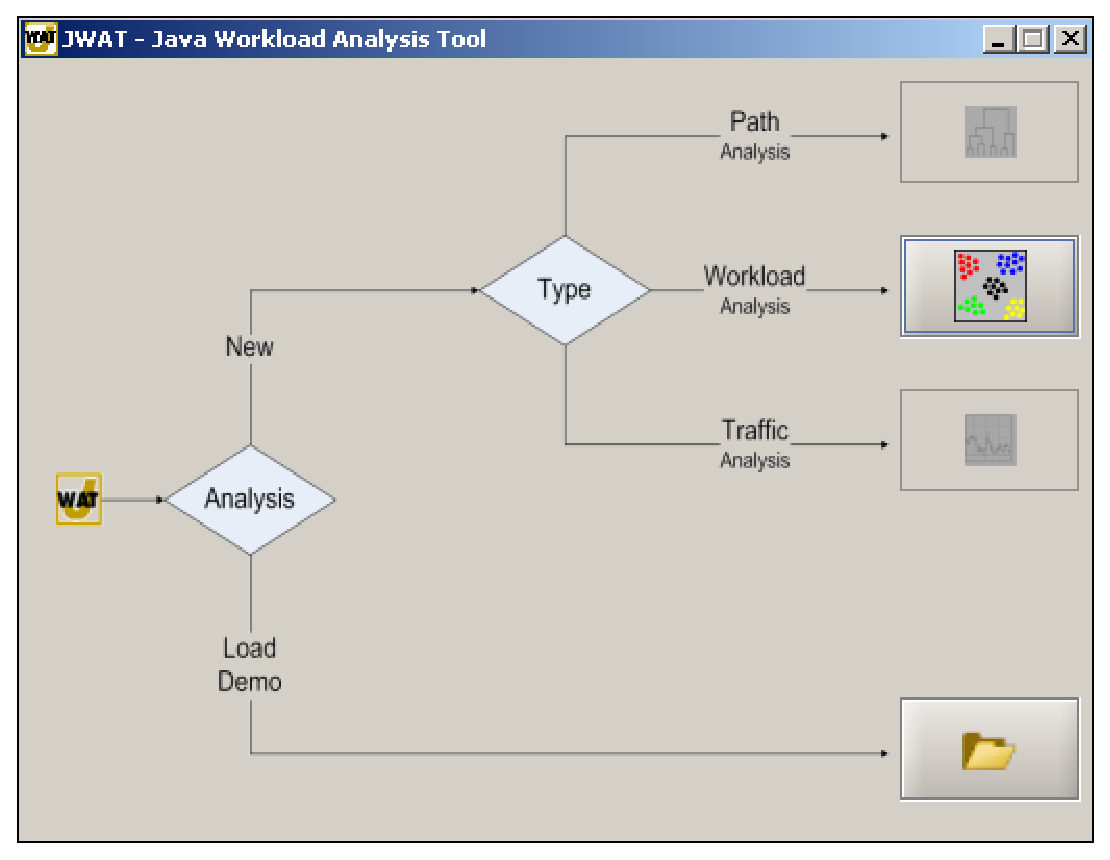
\includegraphics[scale=.6]{img/jwat/Manual/jwat_start_screen.eps}
    \end{center}
    \caption{Main window of JWAT - Workload Analyzer Tool}
    \label{fig:jwat_start_screen}
\end{figure}
Through this window, it is possible to select one of the three
main components of JWAT:

\begin{description}
\item 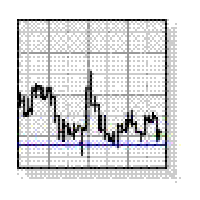
\includegraphics[scale=.2]{img/jwat/TrafficIcon.eps}
\textbf{Traffic Analysis:} Characterization of the arrival traffic
of requests analyzing the timestamp in a log file and deriving the
parameters that refer to the burstiness of requests

\item \includegraphics[scale=.15]{img/jwat/WorkLoadIcon.eps}
\textbf{Workload Analysis:} Characterization of the workload of a
system through the analysis of the log files applying a clustering
algorithm (k-Means or Fuzzy k-Means) and other statistical
techniques. The input data can be loaded directly from standard
log files (e.g., Apache log files, IIS) or from files with any
format described by the users. Several graphical representations
of the results are also provided for their statistical comparison
(histograms, pie-charts, dispersion matrix, QQ-Plot, QQ-Plot
matrix, scatter plots, ...).

\item 
\includegraphics[scale=.3]{img/jwat/PathIcon.eps} \textbf{Path
Analysis:} The navigation paths followed by the users of a web
site allow the identification of the access paths that should be
considered as representatives of the workload analyzed.
\end{description}

\newpage


\section{Workload analysis}
\label{cha:usrman:wla} To perform a workload analysis press the
button
\includegraphics[scale=.18]{img/jwat/Manual/WorkLoadIcon.eps}
 of the JWAT window and the
window of \autoref{fig:wl_start_screen} will be opened.
\begin{figure}[htbp]
    \begin{center}
        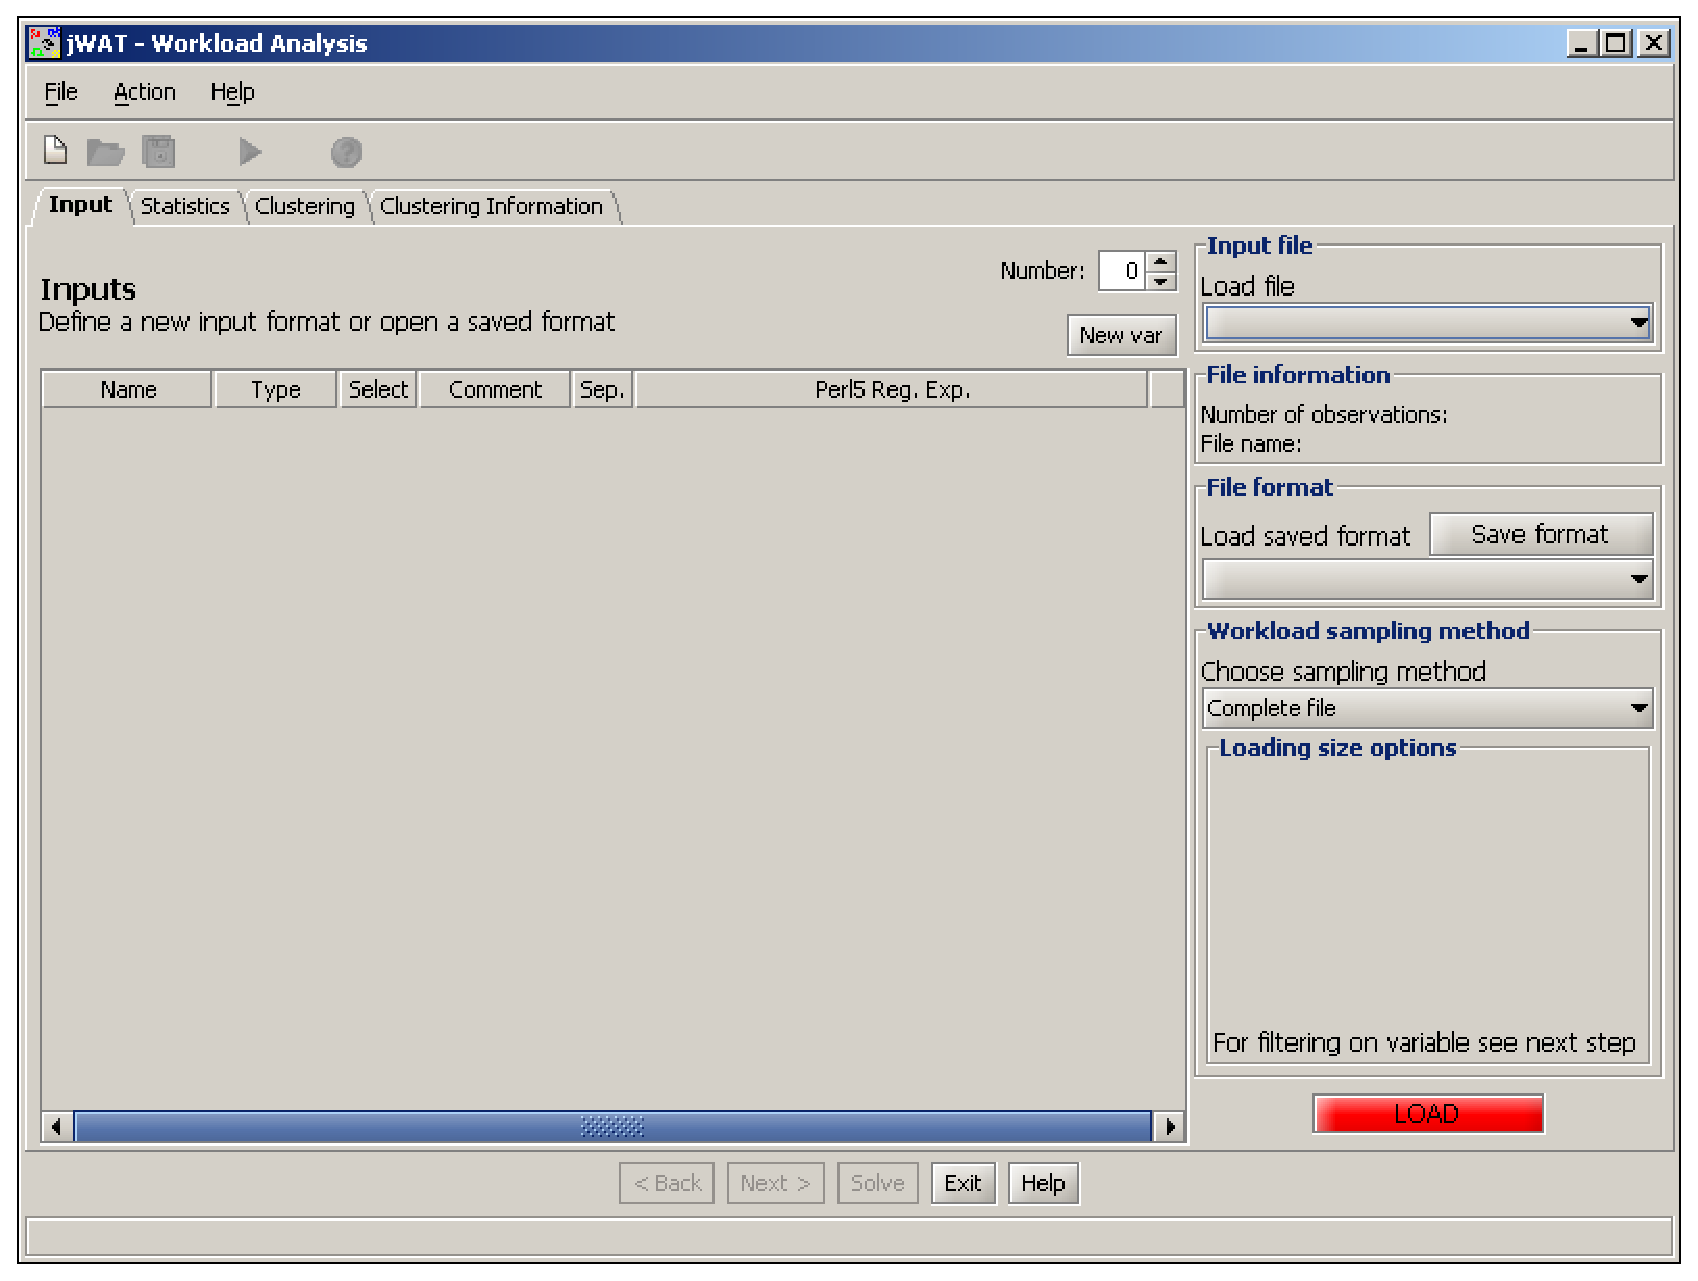
\includegraphics[scale=.5]{img/jwat/Manual/WLStartScreen.eps}
    \end{center}
    \caption{Main window for the Workload analysis}
    \label{fig:wl_start_screen}
\end{figure}
This application help the user to perform in the proper sequence
the various steps of the workload characterization from the data
loading to the statistical analysis, to the results visualization
and to their evaluation. The main components of the workload
analysis window are:
\begin{itemize}
\item \emph{Men�}: three groups of functions are available: File,
Action, Help.
%(\autoref{fig:menu_toolbar}).
To utilize the menu select the desired option. For the description
of menu options see Section \autoref{sec:usrman:desc_menu}. \item
\emph{Toolbar}: several buttons are available
%(\autoref{fig:menu_toolbar})
to facilitate and to speed up the access to the functions (e.g,
New input file, Help ... see Section \autoref{sec:usrman:desc_menu}).
When the cursor is over a button tooltips appear.
\begin{figure}[htbp]
    \begin{center}
        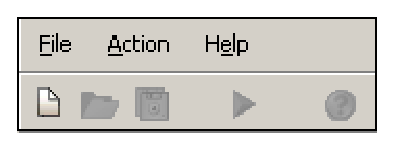
\includegraphics[scale=.5]{img/jwat/Manual/menu_toolbar.eps}
    \end{center}
    \caption{Men� and application toolbar}
    \label{fig:menu_toolbar}
\end{figure}
\item \emph{Tabbed pane}: It concerns the main functions of the
application. All the operations that can be performed on the input
data are shown in four navigable tabs: input, statistics,
clustering, clustering information (\autoref{fig:tabs_all}).
\begin{figure}[htbp]
    \begin{center}
        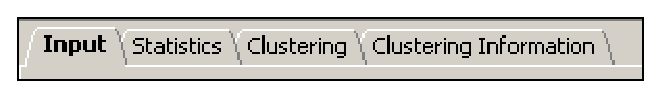
\includegraphics[scale=.5]{img/jwat/Manual/tabs_all.eps}
    \end{center}
    \caption{Tabs selector}
    \label{fig:tabs_all}
\end{figure}
\item \emph{Navigation buttons}: used for navigate between panels.
The buttons are enabled and disabled automatically depending on
the operations to be performed in the actual step (\autoref{fig:nav_button_menu}).
\begin{figure}[htbp]
    \begin{center}
        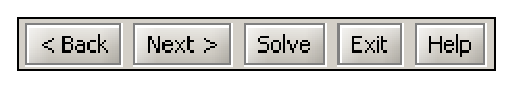
\includegraphics[scale=.5]{img/jwat/Manual/nav_button_menu.eps}
    \end{center}
    \caption{Navigation buttons}
    \label{fig:nav_button_menu}
\end{figure}
\end{itemize}
In the following sections the utilization of the panels  will be
described in detail together with the available options.


\subsection{A workload characterization study}
In this section  the main operations to be performed in a workload
characterization study are described. The definition of the {\it
workload basic components}, that is, the identification of the
smallest level of detail that is to be considered and of the set
of variables to be used for their description, is among the first
operations to be performed. Depending on the intended use of the
study, as workload basic components one may select interactive
commands, database queries and updates, web site requests, web
downloads, programs, scripts, servlets, applets, traffic
intensity, source level instructions, etc. In the following we
will refer to a workload basic component as an {\em observation}
(i.e., an item in the input file) and to the parameters that
describe each component as {\em variables}.
\begin{enumerate}
\item The first step consists of the selection of the file
containing the data that are to be considered as input, of the
variables to load and of their format (see Section~\ref{sec:usrman:sel_def_format}). Let us remark that each
observation may be described in the input file by $n$ variables
but that the number of variables that are considered in the actual
statistical analysis may be less than $n$. It is also possible to
decrease the number of observations of the original input file
(decrease its size) that will be loaded (considered) in the
characterization study. Several filtering criteria for the
construction of a sample of data are available: random selection
of a given number of observations, selection of the observations
that belong to a given interval of their sequence number. At the
end of the data loading a panel describing the errors found in the
data is shown. A user may decide to stop the analysis and verify
the input data or may continue with the following steps.

\item Computation and visualization for each variable of the
descriptive statistics univariate and bivariate, of the frequency
graphs, of the scatter plots, and of the QQ-plot compared to a
normal or exponential distribution (Section~\ref{cha:usrman:stat}).\\
It is important to observe that usually the variables are
expressed in nonhomogeneous units. To make them comparable a
\emph{scale change} must be performed. The following statistical
analysis of the original data, especially of the histograms of
their parameters, allows us to determine when it would be useful
to apply to them a logarithmic or another transformation. Very
often the density functions of some variables are highly
positively skewed and have high values of kurtosis too. Applying a
logarithmic transformation of highly skewed variable densities it
is possible to avoid or to reduce correlations among means and
variances of the clusters that will be identified. Several {\em
transformations} may be applied to the numeric variables
(attention, {\em ONLY} to the numeric variables)
.\\
A {\em sample} may be extracted from input file by using different
criteria. The distributions of two variables may be compared
through QQ-plots and scatter plots selected in the corresponding
matrix. \item Selection of the clustering algorithm to apply and
of the variables to be considered in the cluster analysis (see
Section~\ref{cha:usrman:kmean}). The basic idea is to partition
the given set of observations into classes of components having
homogeneous characteristics. Among the various clustering
algorithms the most commonly applied to workload characterization
problems belong to the non-hierarchical k-means family. The
algorithm produces a number of classes ranging from 1 to $k$,
where $k$ is a parameter that must be specified by the user. The
observations are assigned to a class so that the sum of the
distances between all the elements and the centroid of the class
is minimized. A set of representative components will then be
selected from the classes according to some extraction criteria
(usually the centroids of the clusters) and used in the
construction of the workload model. \item A panel is available for
the visualization of the results of the clustering analysis.
Several graphics and tables are reported in order to describe the
clusters composition and the goodness of a partition. Scatter
plots are available for all the variables considered (see Section~\ref{cha:usrman:rkmean}).
\end{enumerate}
\subsection{Input definition}
The panel for the description of the input data 
(\autoref{fig:wl_start_screen}) is a very important one since it allows
the selection of the input file that contains the data to be
analyzed and the description of their structure. In such a way we
may take into consideration the log files generated by different
systems and tools. The format definition structure of the input
file is described in detail in Section
\autoref{sec:usrman:es_def_form}.
\subsubsection{Input file selection}
\label{cha:usrman:selinp} To select the input file use the panel
shown in 
 \autoref{fig:input_browse}. The \emph{Browse...} option for the selection of the
 input file is available (\autoref{fig:input_browse}).
 Once a file has been selected its name is added to the list of the files available for
 following analyses.
\begin{figure}[htbp]
\begin{center}
        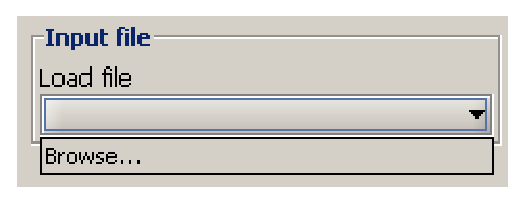
\includegraphics[scale=.5]{img/jwat/Manual/input_browse.eps}
    \end{center}
    \caption{Panel for the selection of the input file}
    \label{fig:input_browse}
\end{figure}
A panel showing the number of observations loaded and the file
name will automatically appears (\autoref{fig:file_information}).
\begin{figure}[htbp]
\begin{center}
        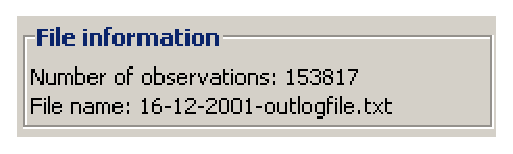
\includegraphics[scale=.7]{img/jwat/Manual/file_information.eps}
    \end{center}
    \caption{Panel with information about the selected file}
    \label{fig:file_information}
\end{figure}
\subsubsection{Format definition}
\label{sec:usrman:sel_def_format} The next operation consists of
the definition of the data format. The format of the input data is
required by the application:
\begin{itemize}
\item to recognize the number of variables that belongs to each
observation \item to recognize the type (string, numeric or data)
of each variable \item to the right interpretation of the meaning
of each data element that belong to a single observation. For the
definition of the elements regular expressions Perl5 (Section
\autoref{sec:usrman:es_def_form}) are used. The defined formats are
stored in a library and can be browsed and reused.
 \item to select a subset of the variables of the observations that are in the original input file.
\end{itemize}
We will describe a very simple example of the format definition of
an '\emph{observation}, i.e., a single element in the input log
file. The considered log file contains several data, e.g., IP
client address that submits the request for a resource to a web
server, request timestamp,  etc...) that are called
\emph{variables}.

After the selection of the input file, the format definition table
is empty, see \autoref{fig:wl_start_screen}, since no
information regarding current format has already been defined.

Two types of format definition are available:
\begin{itemize}
\item Manual, that consists of the definition of the format of
each single variable through relative table and relative commands
\item Automatic, that load one of the predefined standard formats
previously defined and loaded in files \emph{`.jwatformat'}.
\end{itemize}
\subsubsection{Manual definition}
\label{sec:usrman:sel_def_format:man} At the beginning, the
correct number of variables of each observation in the log file is
to be set (use the spinner \emph{`Number'}). By using the
`\emph{New var}' button a new variable is added  to the format
table. The same result is obtained using the spinner
\emph{`Number'} at the right top of the table (see \autoref{fig:manual_format}).

To remove one or more variables by a format table we can utilize:
\begin{itemize}
\item the button

\includegraphics[scale=.8]{img/jwat/Manual/del_button.eps}
at the end of each row of the table. The result is the deletion of
the concerning variable \item turned arrow towards the bottom of
the spinner. The result is the deletion of the last variable of
the table \item the right button of the mouse on a single selected
variable, or on a set, to delete them from the format table
(\autoref{fig:mouse_del_var}).
\end{itemize}
%\begin{figure}[htbp]
%\begin{center}
%        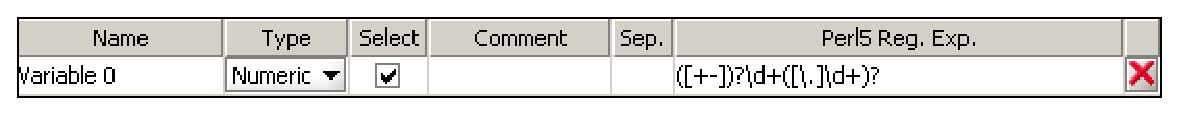
\includegraphics[scale=.5]{img/jwat/Manual/single_row.eps}
%    \end{center}
%    \caption{Format table row}
%    \label{fig:single_row}
%\end{figure}
\begin{figure}[htbp]
\begin{center}
        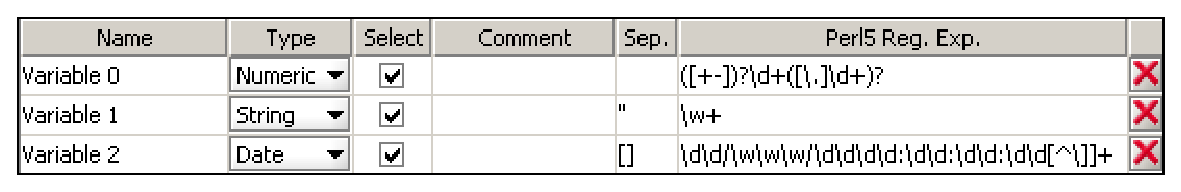
\includegraphics[scale=.5]{img/jwat/Manual/manual_format.eps}
    \end{center}
    \caption{Format table}
    \label{fig:manual_format}
\end{figure}
\begin{figure}[htbp]
\begin{center}
        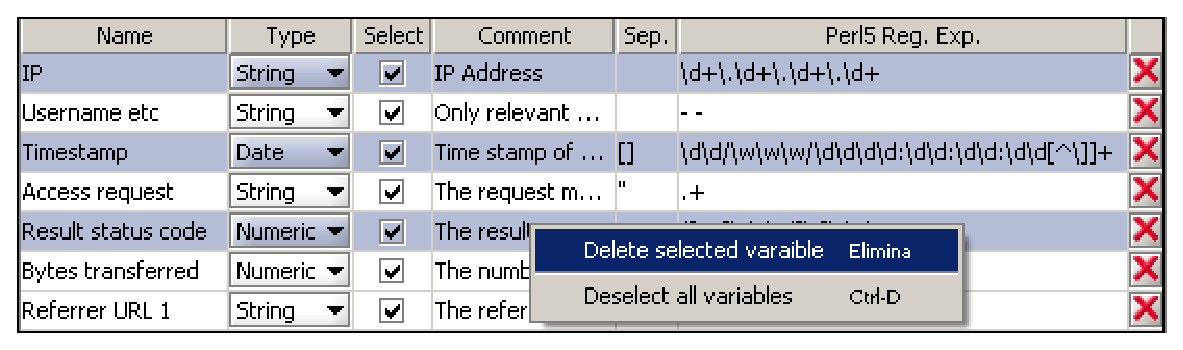
\includegraphics[scale=.5]{img/jwat/Manual/mouse_del_var.eps}
    \end{center}
    \caption{Deletion of selected variables}
    \label{fig:mouse_del_var}
\end{figure}
Once the correct number of variables in a observation is defined
the next step is their description. The columns of the format
table have the following meaning:
\begin{itemize}
\item \emph{Name:} as default, to each new added variable it is
assigned the standard name \emph{Variable X}. In order to
facilitate the analysis of the results it is recommended to change
these names with new ones related with the meaning of the
variables. \item \emph{Type:} it identifies the type of the
variable. Possible choices are \emph{number, string} and
\emph{data}. The type definition is fundamental for the right
interpretation of the results. \item \emph{Selection:} it allows
to specify which of the variables of the observations registered
in the input file will be effectively loaded. In any case, it is
necessary to define all the variables of each observation, also if
some of them will not be selected for the statistical analysis.
\item \emph{Comment:} it is allowed to add a string of comment to
each variable. \item \emph{Delimiter [Sep]:} it identifies the
character used (if it exists) in the input file to delimit the
field identified by the current variable. For example in the
Apache server log file the variable "timestamp" is contained
within square brackets. \item \emph{Regular Expression :}
definition of regular expression (Perl 5) that defines the
variable. For example in case of IP variables a possible regular
expression is:
`\emph{$\backslash$d+$\backslash$.$\backslash$d+$\backslash$.$\backslash$d+$\backslash$.$\backslash$d+}'.
\item \emph{Delete:} the corresponding variable will be deleted.
\end{itemize}

In order to help the users for each of the types the tool sets
automatically some of the fields (delimiter of field and regular
expression) supplying standard settings as shown in 
\autoref{fig:manual_format} where for for the type \emph{string} it is
proposed '' as delimiter and $\backslash$w+ as regular expression.

A format definition may be saved by using the `\emph{Save format}'
button so that it may reused in the future.
\subsubsection{Format loading}
If a standard log file (Apache, IIS) is used it is possible to
load the corresponding format by using the combobox in the panel
of \autoref{fig:file_format}.
\begin{figure}[htbp]
\begin{center}
        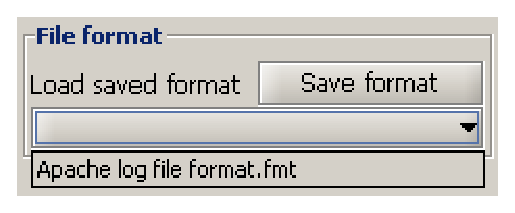
\includegraphics[scale=.5]{img/jwat/Manual/file_format.eps}
    \end{center}
    \caption{Panel for the loading of standard and previously saved format}
    \label{fig:file_format}
\end{figure}\\
For example, by selecting the option ``Apache log file format'',
the format definition table of 
\autoref{fig:input_table_format_apache} is automatically loaded.
\begin{figure}[htbp]
\begin{center}
    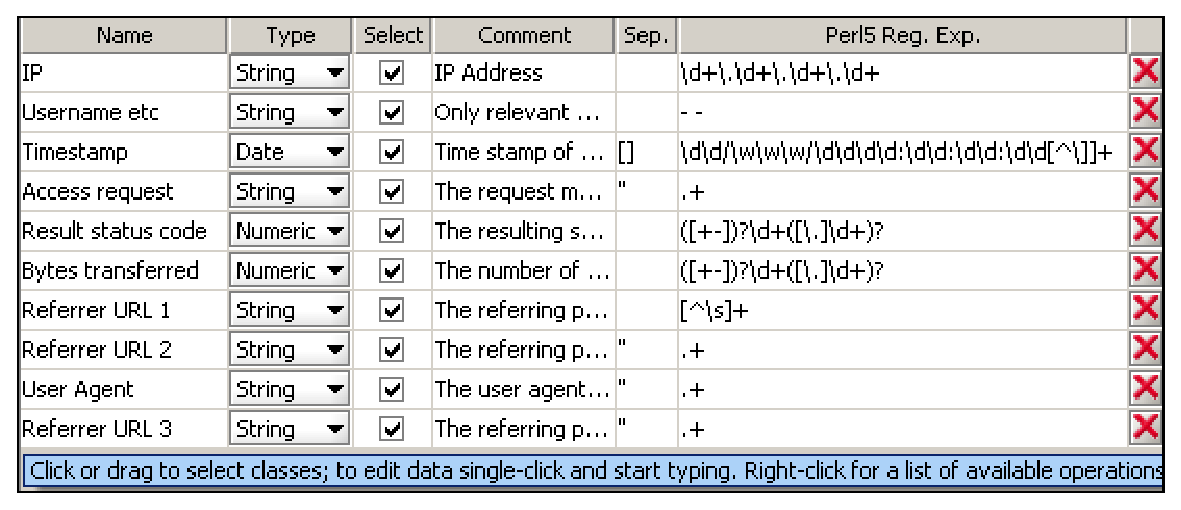
\includegraphics[scale=.5]{img/jwat/Manual/input_table_format_apache.eps}
\end{center}
    \caption{Format definition table}
    \label{fig:input_table_format_apache}
\end{figure}
At this point, the user can select through the format table
selection field the subset of variables to load.
\subsubsection{Methods for extracting a sample}
\label{cha:usrman:sampmet}In order to process the data from real
log files, that usually are constituted by a very large number of
observations (e.g., several Gigabytes), by a cluster algorithm
with a reasonable amount of processing time and storage
dimensions, the size of the original data set has to be reduced.
Thus, only a sample drawn from the original set of data is often
submitted as input to the clustering algorithm.

After the definition of the data format it is possible through the
panel \emph{Workload sampling method} of 
\autoref{fig:sampling_methods}
\begin{figure}[htbp]
\begin{center}
    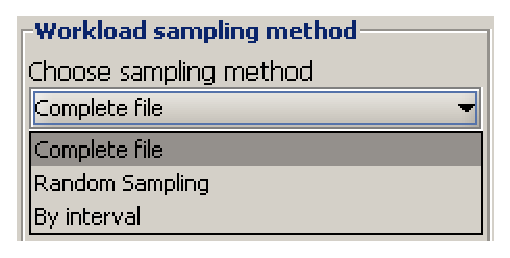
\includegraphics[scale=.5]{img/jwat/Manual/sampling_methods.eps}
\end{center}
    \caption{Extraction criteria for the sample construction}
    \label{fig:sampling_methods}
\end{figure}
 to select one of the following
extraction criteria:
\begin{itemize}

\item \emph{Complete file:} all the observations of the input file
are considered. \item \emph{Random:} the number of observations to
be loaded should be specified in the panel of
Fig.\autoref{fig:sampling_methods_random}.
\begin{figure}[htbp]
\begin{center}
        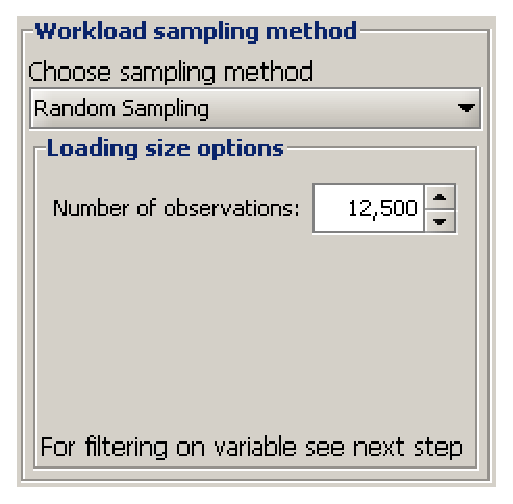
\includegraphics[scale=.5]{img/jwat/Manual/sampling_methods_random.eps}
    \end{center}
    \caption{Random method for the construction of a sample}
    \label{fig:sampling_methods_random}
\end{figure}
\item \emph{Interval:} the panel of 
\autoref{fig:sampling_methods_interval} that requires to specify the
interval of observations (according to their id numbers) to load
will be shown.
\begin{figure}[htbp]
\begin{center}
        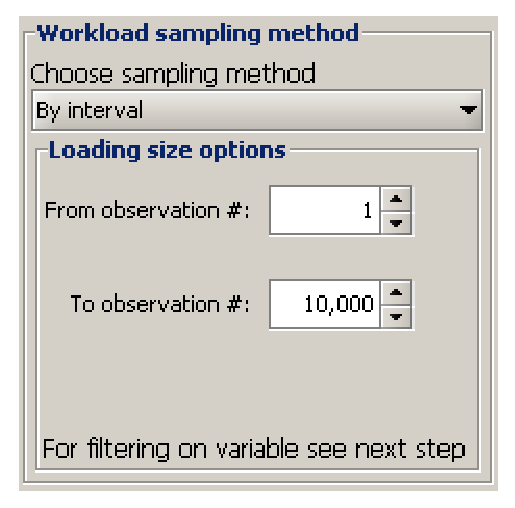
\includegraphics[scale=.5]{img/jwat/Manual/sampling_methods_interval.eps}
    \end{center}
    \caption{Interval method options}
    \label{fig:sampling_methods_interval}
\end{figure}
\end{itemize}

\subsubsection{Loading of log file}
\label{cha:usrman:load} After the definition of the input file the
loading of the selected observations will be started. After
pressing the `\emph{LOAD}' button (\autoref{fig:load_button})
 the loading window of \autoref{fig:load_panel} will be opened.
The percentage of loading completion, the number of processed
observations and the number of
 observations discarded because not consistent with the
specified format are shown.
\begin{figure}[htbp]
\begin{center}
    
\includegraphics[scale=.5]{img/jwat/Manual/load_button.eps}
\end{center}
    \caption{Button for the loading of the input data.}
    \label{fig:load_button}
\end{figure}
\begin{figure}[htbp]
\begin{center}
    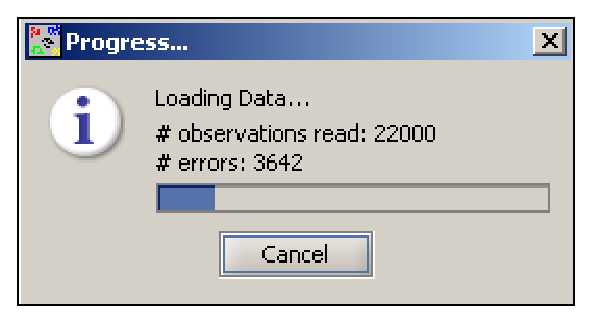
\includegraphics[scale=.5]{img/jwat/Manual/load_panel.eps}
\end{center}
    \caption{Window showing the loading progress}
    \label{fig:load_panel}
\end{figure}
At the end of the load a window summarizing the total number of
observations loaded and the total number of observations loaded
correctly (\autoref{fig:load_complete}) is shown.
\begin{figure}[htbp]
\begin{center}
    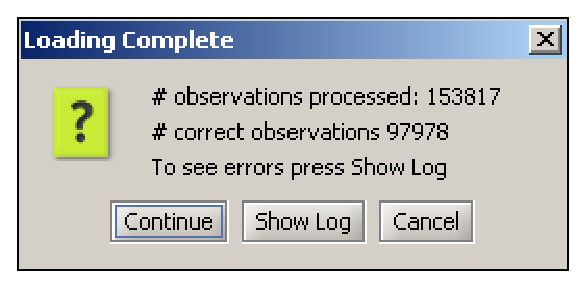
\includegraphics[scale=.5]{img/jwat/Manual/load_complete.eps}
\end{center}
    \caption{Loading phase results}
    \label{fig:load_complete}
\end{figure}
It is possible to visualize the log file that contains the
description of the errors found during the loading operation
(\autoref{fig:error_log}).
\begin{figure}[htbp]
\begin{center}
    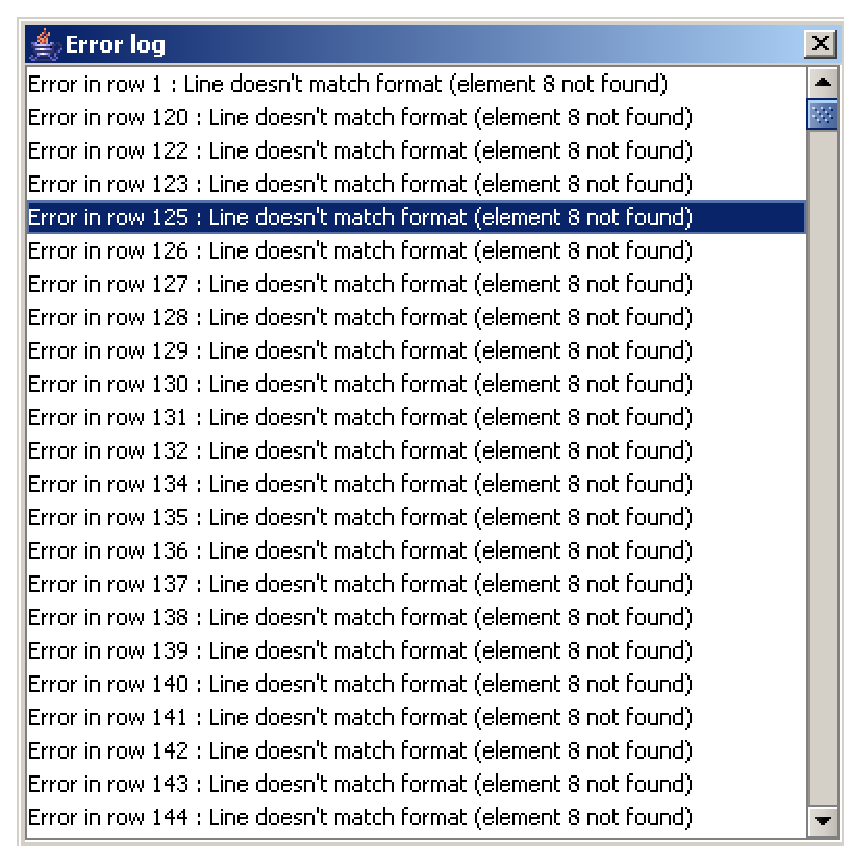
\includegraphics[scale=.5]{img/jwat/Manual/error_log.eps}
\end{center}
    \caption{Example of error log in the loading phase}
    \label{fig:error_log}
\end{figure}
The error messages that are contained in the log file are:
\begin{itemize}
\item \emph{Error in row xx : Element y is wrong}: (if you defined
separators) the element corresponding to the variable \emph{y},
for the row \emph{xx}, does not correspond to the defined regular
expression. \item \emph{Error in row xx : Line does not match
format (element y not found)}: The element corresponding to the
variable \emph{y} is not present in the row (observation)
\emph{xx} of the input file. \item \emph{Error in row xx : Too
many fields} : the row \emph{xx} contains elements in excess
compared to the defined format. This may indicate with high
probability that the format definition described by the user is
not correct for the considered observation.
\end{itemize}
\subsection{Data processing}
A tabs substructure (\autoref{fig:stat_tabs}) shows the groups
of the various statistics available:
\begin{description}
\item[Univariate: ] descriptive statistics, graphs and
transformations. \item[Sample construction: ] methods of sample
construction and data filtering. \item[Bivariate: ] bivariate
statistics. \item[QQ-plot matrix: ] QQ-plots of the variables for
comparison with normal and exponential distributions \item[Scatter
plot matrix: ] Scatter plots of all the variables.
\end{description}
\begin{figure}[htbp]
\begin{center}
    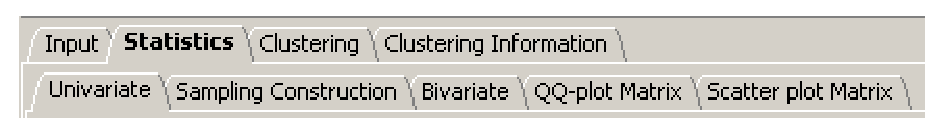
\includegraphics[scale=.5]{img/jwat/Manual/stat_tabs.eps}
\end{center}
    \caption{Tabs structure for the processing of the data}
    \label{fig:stat_tabs}
\end{figure}
\subsubsection{Statistics}
\label{cha:usrman:stat} The univariate and bivariate panels show
respectively several statistical indexes concerning each variable
of the observations (\autoref{fig:univ_stats}) and the
correlation coefficients of the variables (\autoref{fig:biv_stats}).
\begin{figure}[htbp]
\begin{center}
    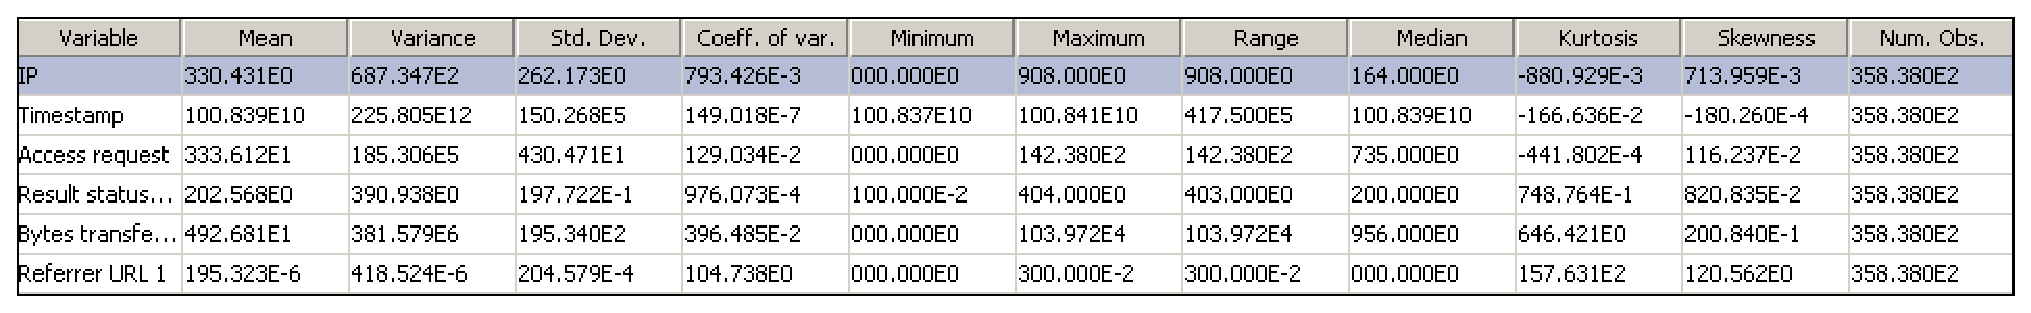
\includegraphics[scale=.5]{img/jwat/Manual/univ_stats.eps}
\end{center}
    \caption{Descriptive statistics of the variables}
    \label{fig:univ_stats}
\end{figure}
\begin{figure}[htbp]
\begin{center}
    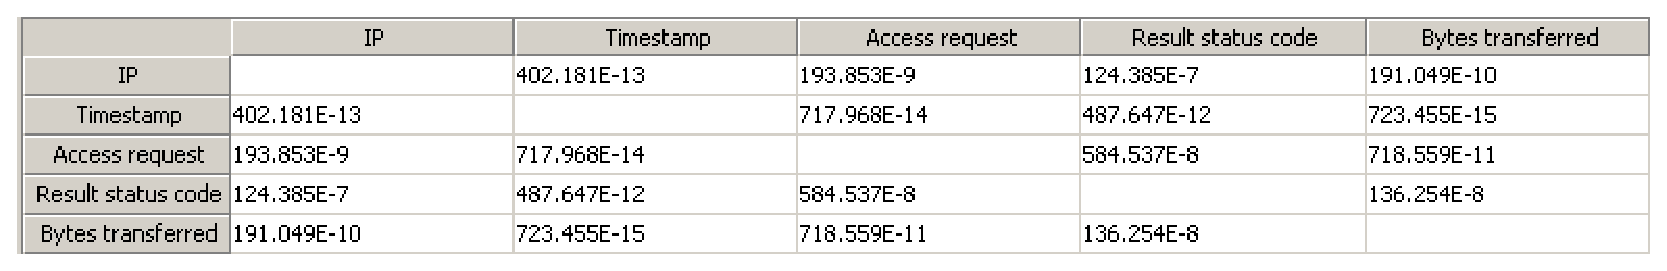
\includegraphics[scale=.5]{img/jwat/Manual/biv_stats.eps}
\end{center}
    \caption{Correlation coefficients of the variables}
    \label{fig:biv_stats}
\end{figure}\\
The univariate panel shows also the following two types of graphs:
\begin{itemize}
\item a histogram, or frequency graph, preview for each variable,
that can be magnified with a double click on the preview (\autoref{fig:histogram}).
\begin{figure}[htbp]
\begin{center}
    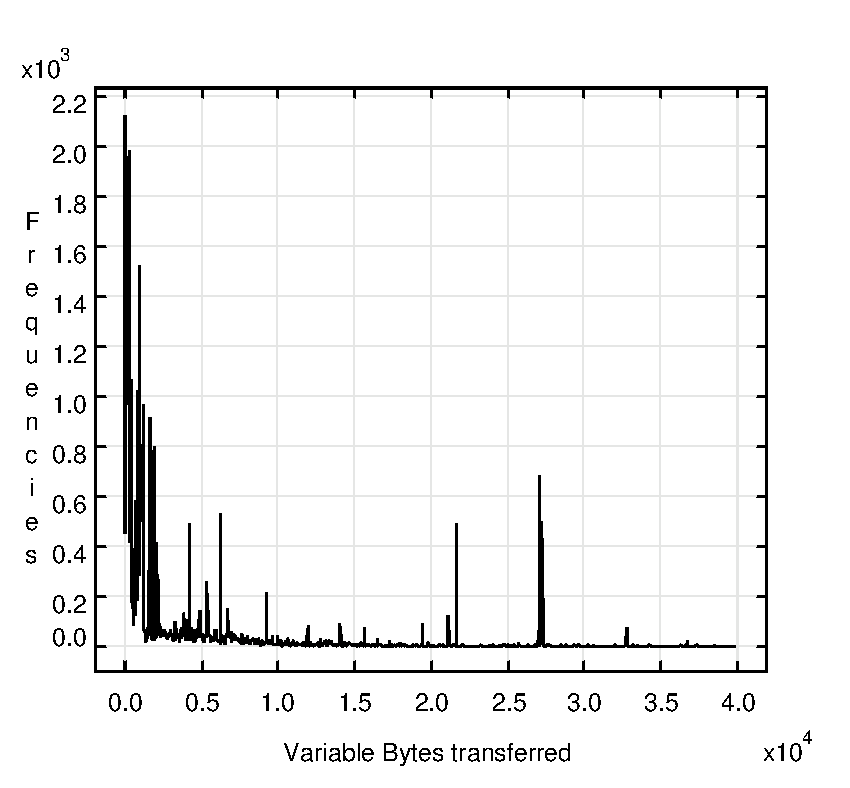
\includegraphics[scale=.5]{img/jwat/Manual/histogram.eps}
\end{center}
    \caption{Histogram, or frequency graph, of the variable "Bytes transferred"}
    \label{fig:histogram}
\end{figure}
\item a preview of the QQ-plot graph of the variable quantiles
compared with the normal distribution quantiles with the same
average and variance or the exponential distribution with the same
average. Also this preview can be magnified with a double click
(\autoref{fig:qqplot_prev}).
\end{itemize}
\begin{figure}[htbp]
\begin{center}
    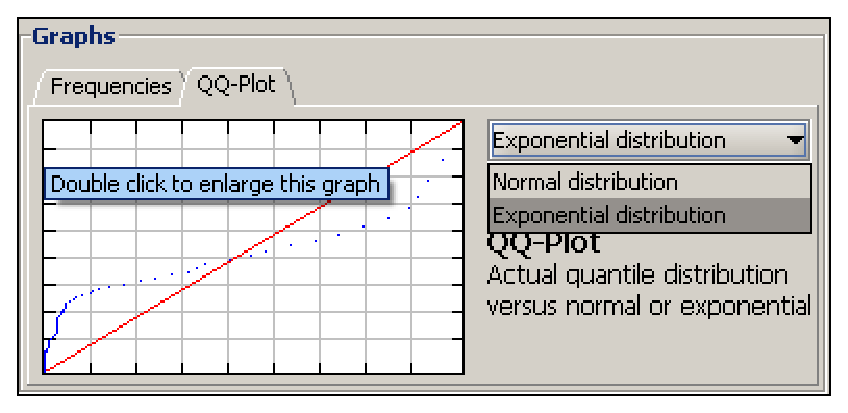
\includegraphics[scale=.5]{img/jwat/Manual/qqplot_prev.eps}
\end{center}
    \caption{QQ-plot preview for the comparison of a given distribution
    with an exponential or a normal ones.}
    \label{fig:qqplot_prev}
\end{figure}
Both magnified graphs can be saved in \emph{eps} (Encapsulated
PostScript) and \emph{png} (Portable Network Graphics) formats.

\subsubsection{Transformations and sample extraction}
\label{cha:usrman:tras} The panel of univariate statistics allows
also to perform some variables transformations. To apply a
transformation select the variable in the table of 
\autoref{fig:univ_stats}; if it is of a numeric type the panel of
\autoref{fig:transf_panel} that allows the selection of the
type of transformation (logarithmic, min-max and standard
deviation)  will be shown and press the `\emph{Apply
transformation}' button. It is possible to undo the last
transformation by pressing the `\emph{Undo transformation}'
button. The list of the variables with the transformations applied
is reported in the table. If the selected variable is not numeric,
the following message is shown: \emph{``This variable could not be
transformed since it is not numeric''}.
\begin{figure}[htbp]
\begin{center}
    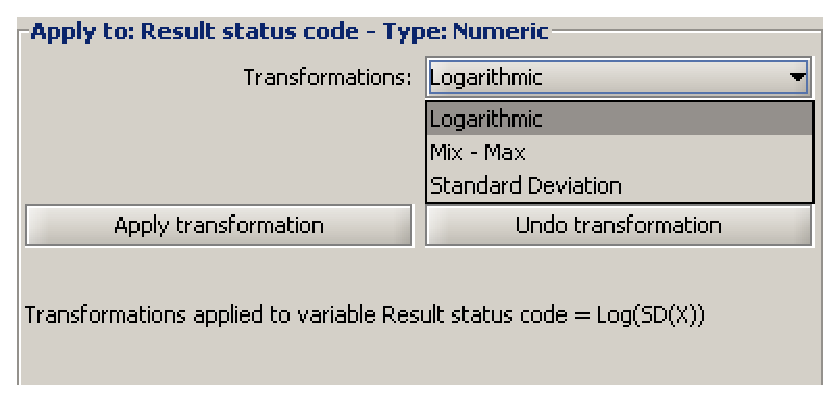
\includegraphics[scale=.5]{img/jwat/Manual/transf_panel.eps}
\end{center}
    \caption{Selection of the transformation to apply to the original data}
    \label{fig:transf_panel}
\end{figure}

To extract a sample from the original input file press on tab
\emph{`Sample construction'}. The panel of
\autoref{fig:filters_list} shows the possible criteria that can be
applied to the loaded variables that depends on the selected
method and on the type of the variables.
\begin{figure}[htbp]
\begin{center}
    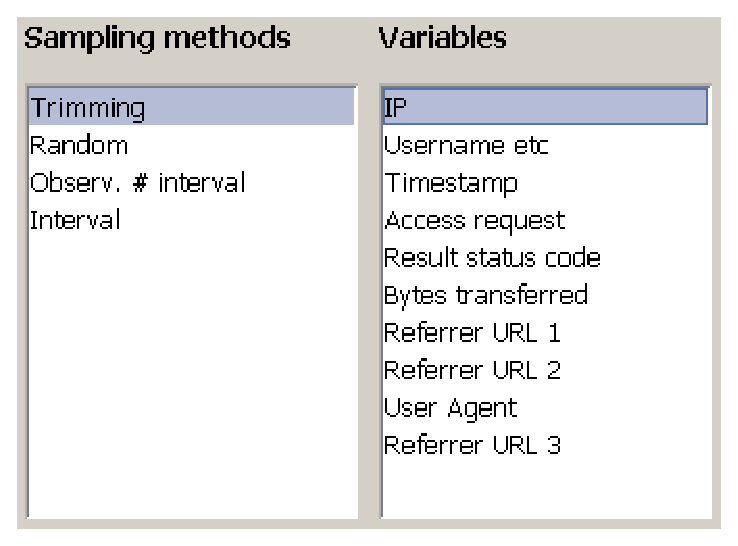
\includegraphics[scale=.5]{img/jwat/Manual/filters_list.eps}
\end{center}
    \caption{Sampling extraction criteria that can be applied on the selected variables}
    \label{fig:filters_list}
\end{figure}

\begin{itemize}
\item \emph{Random} and \emph{Obsev. \# interval} methods are
similar to those available in input window and allow to select
randomly \emph{n} observations from the input file or to extract
the observations whose numerical identifiers are included into the
interval defined by the user.

\item \emph{Trimming :} the outliers, i.e., those values of a
variable that are too distant from the other values of the same
variable, may distort the transformation and the statistical
analysis by causing the other observations to be assigned too much
or too little weight should be removed.  To filter a variable
distribution (trimming operation) the percentiles that should be
removed can be specified (\autoref{fig:trimming}).
\begin{figure}[htbp]
\begin{center}
    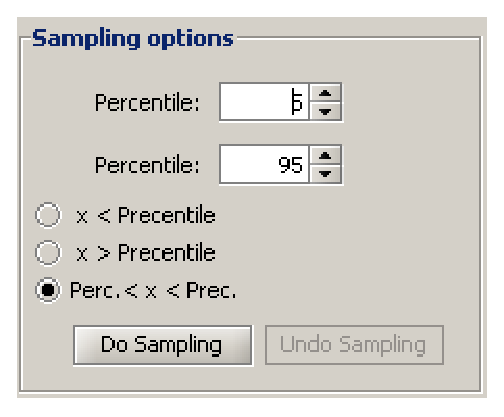
\includegraphics[scale=.5]{img/jwat/Manual/trimming.eps}
\end{center}
    \caption{Filter of the percentiles of a variable (trimming of the distribution)}
    \label{fig:trimming}
\end{figure}

\item \emph{Interval} operation applies a filter on a variable's
values. Depending on the type of the variable different options
panels will be shown. If the selected variable is \emph{numeric}
the panel is similar to that of \autoref{fig:num_filter}: the
minimum and maximum values of the variable should be specified. If
the selected variable is of \emph{data} type the panel is similar
to that of \autoref{fig:time_filter}: the dates of start and
end of observations should be specified. If the variable is of
\emph{string} type, it is possible to specify a substring that has
to be contained in the selected observations.
\begin{figure}[htbp]
\begin{center}
    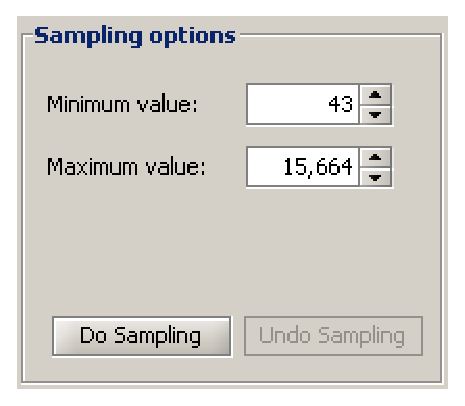
\includegraphics[scale=.5]{img/jwat/Manual/num_filter.eps}
\end{center}
    \caption{Filter on the values of a numeric variable}
    \label{fig:num_filter}
\end{figure}
\begin{figure}[htbp]
\begin{center}
    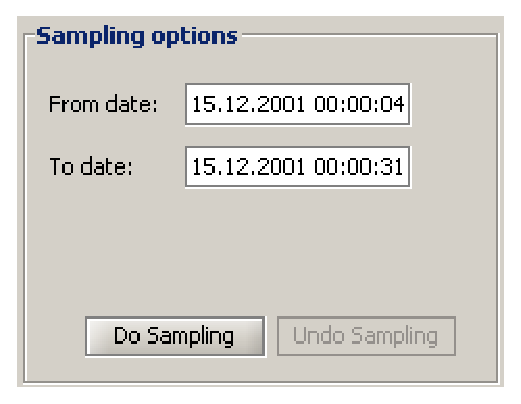
\includegraphics[scale=.5]{img/jwat/Manual/time_filter.eps}
\end{center}
    \caption{Filter on the values of a data variable}
    \label{fig:time_filter}
\end{figure}
\end{itemize}
The operation of \emph{`Undo sampling'} is available.
\subsubsection{Graphs}
\label{cha:usrman:grap} The last two panels of the statistics tab
concern a preview of QQ-plot graphs and of scatter plots for all
the variables, respectively. Both allow to save graphs in the most
common formats(\emph{.png, .eps}). Previews can be magnified with
a left double click of the mouse. Several functions are available
for the graphs: portions zoom, points dimension, by clicking the
right button of the mouse on a graph various formats are available
for export the graph as image.
%\begin{multicols}{2}
\begin{figure}[htbp]
    \begin{center}
        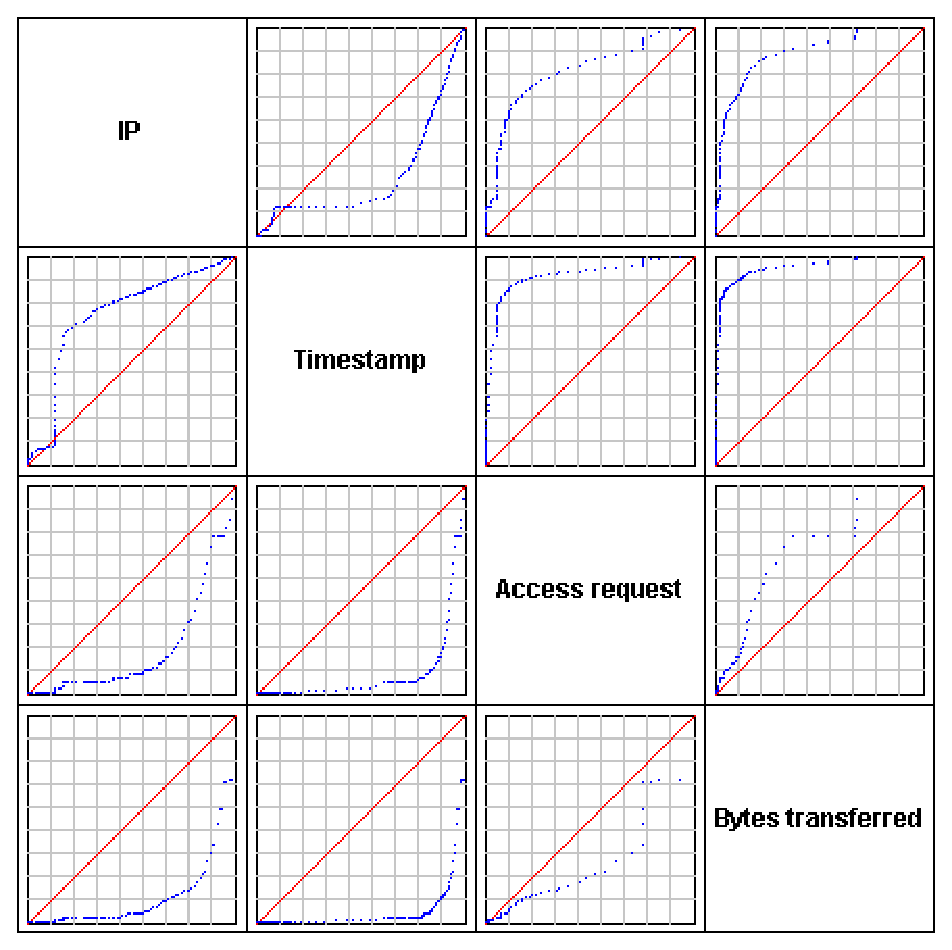
\includegraphics[scale=.6]{img/jwat/Manual/qqplot_matrix.eps}
        \ \\
        \ \\
        \caption{QQ-plot matrix for the comparison of the distributions
        of two variables}
        \label{fig:qqplot_matrix}
    \end{center}
\end{figure}
%\columnbreak
\begin{figure}[htbp]
    \begin{center}
        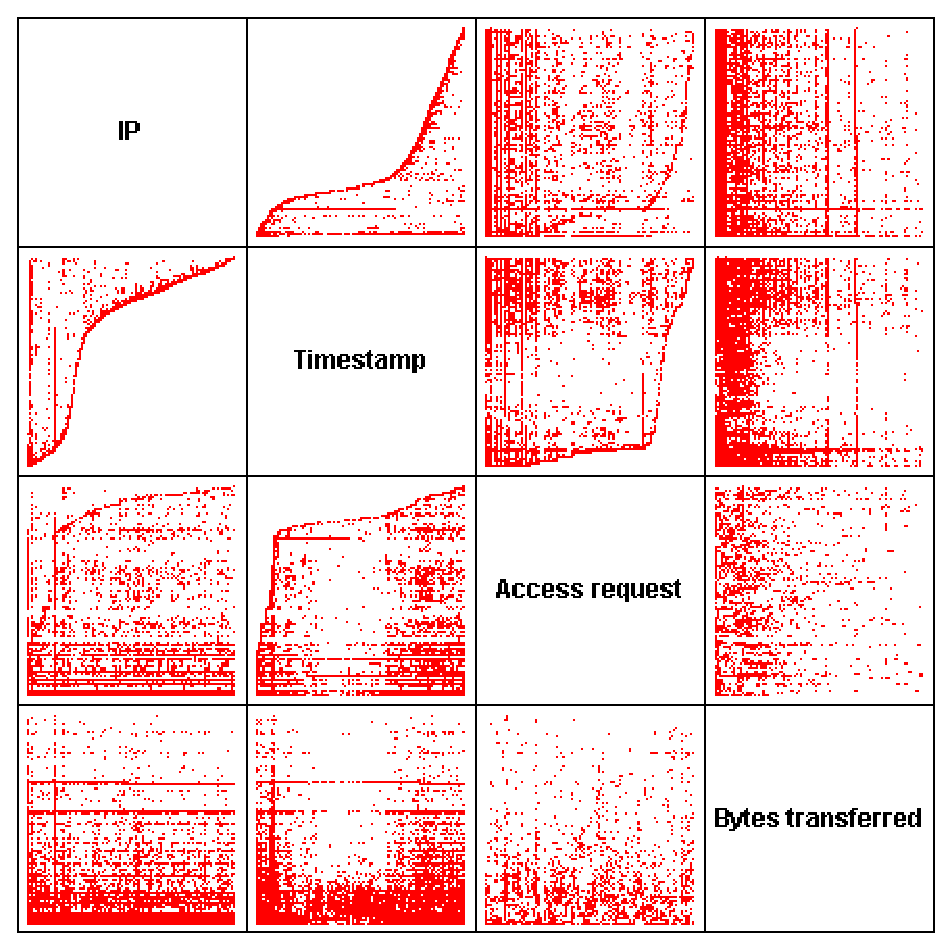
\includegraphics[scale=.6]{img/jwat/Manual/scatter_matrix.eps}
        \ \\
        \ \\
        \caption{Scatter matrix}
        \label{fig:scatter_matrix}
    \end{center}
\end{figure}
%\end{multicols}
\subsection{Clustering algorithms}
The next step of the characterization process is the choice of the
clustering algorithm to be used ad of the options available. Two
clustering algorithms are actually implemented in the tool
(k-Means and Fuzzy k-Means), see \autoref{fig:cluster_lists}.
Depending on the selected algorithm, in the right panel of tab the
available options are listed.

The execution of a clustering algorithm will start when the
buttons `\emph{Solve}' or
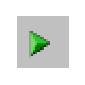
\includegraphics[scale=.5]{img/jwat/Manual/Sim.eps} are pressed.
During the execution, the window of \autoref{fig:clust_load}
that report the progress state and allows to interrupt the
execution is shown.
\begin{figure}[htbp]
\begin{center}
    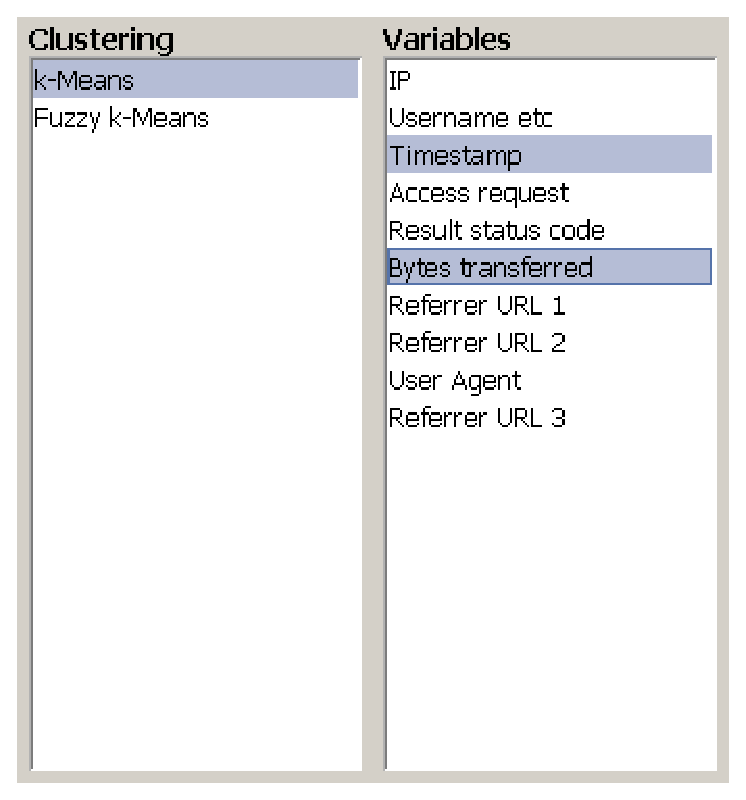
\includegraphics[scale=.5]{img/jwat/Manual/cluster_lists.eps}
\end{center}
    \caption{Clustering algorithm used and variables selected that will be
    considered in the analysis.}
    \label{fig:cluster_lists}
\end{figure}
\begin{figure}[htbp]
\begin{center}
    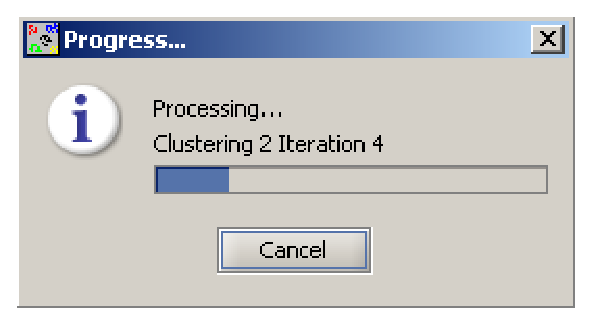
\includegraphics[scale=.5]{img/jwat/Manual/clust_load.eps}
\end{center}
    \caption{Clustering progress panel}
    \label{fig:clust_load}
\end{figure}
\subsubsection{K-Means algorithm}
\label{cha:usrman:kmean} The non-hierarchical k-Means algorithm
implemented in the tool requires the specification of the
following parameters, \autoref{fig:kmeans_options}:
\begin{itemize}
\item \emph{the maximum number k of clusters} that the algorithm
has to produce. Note that the algorithm produces the results for
all partitions from 1 to $k$ clusters \item \emph{the maximum
number of iterations} to perform in order to find the optimal
partition. The initial subdivision into $k$ clusters is
iteratively improved by shifting, based on the selected criterion
(in this case the Euclidean distance), the elements of a cluster
to another and computing after each assignment the new center of
mass of the clusters. The optimum configuration is obtained when
points can no longer be reassigned. The selected value is an upper
limit of the number of interactions for each partition.
Experiences suggest the value of 4 interactions as a reasonable
choice: the results are obtained in a short time and are enough
accurate. To obtain more accurate results higher values should be
used, this involves a higher computation time \item \emph{the
transformation type} to apply to selected variables (if needed).
Transformations of the values are applied before the execution of
the algorithm and at the end of the execution the results can be
transformed back to their original values. The transformation of
the values is often required since the variables are usually
expressed in different units and their ranges are very different.
Since the algorithm uses the Euclidean distance function as
comparison metric to determine if an observation belongs to a
cluster, the results could be not reliable if the values differ of
one or more order of magnitude.
\end{itemize}
\begin{figure}[htbp]
\begin{center}
    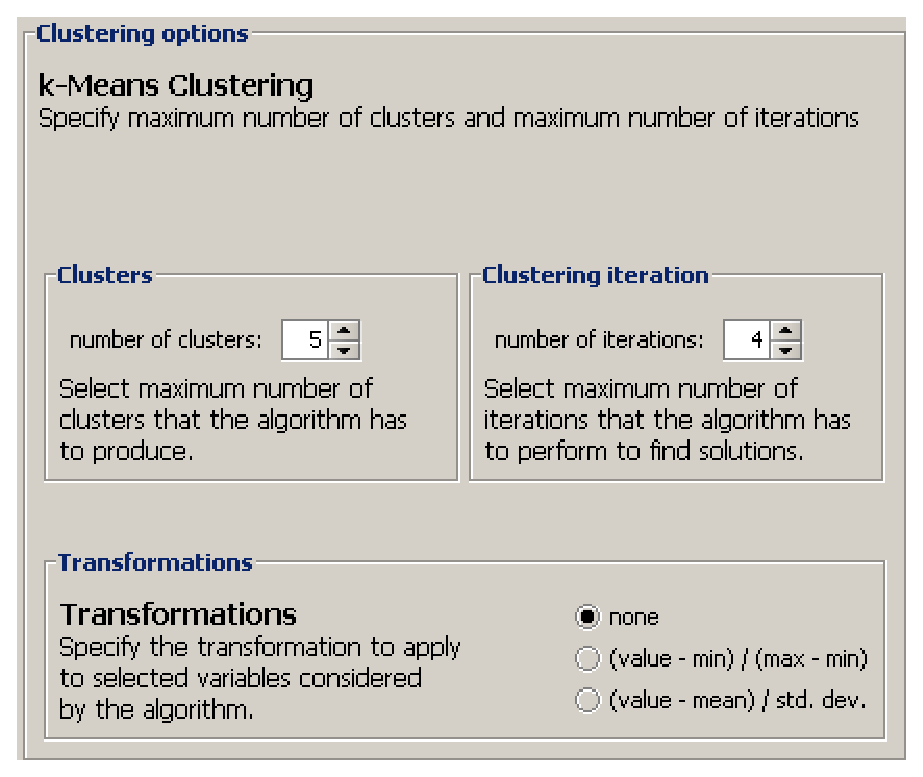
\includegraphics[scale=.5]{img/jwat/Manual/kmeans_options.eps}
\end{center}
    \caption{Parameters of the clustering algorithm k-Means}
    \label{fig:kmeans_options}
\end{figure}
\subsubsection{Fuzzy k-Means algorithm}
\label{cha:usrman:fuzzy} The fuzzy k-Means algorithm implemented
in the tool requires the following parameters,
\autoref{fig:fuzzy_options}:
\begin{itemize}
\item \emph{the maximum number k of clusters} that the algorithm
has to produce. The results for all the partitions from two to the
selected maximum value will be provided. The higher is this value
the higher is the execution time of the algorithm \item \emph{the
maximum number of iterations} to perform in order to find the
optimal partition. Four is a suggested value. See the comments
reported above for the K-means algorithm.  \item \emph{the
fuzziness level} to apply during the algorithm execution. It is
the value used by algorithm to determine the fuzziness degree of
final solution. It ranges from 2 to 100 \item \emph{the
transformation type} to apply to selected variables (if needed).
See the comments reported above for the K-means algorithm.
\end{itemize}
\begin{figure}[htbp]
\begin{center}
    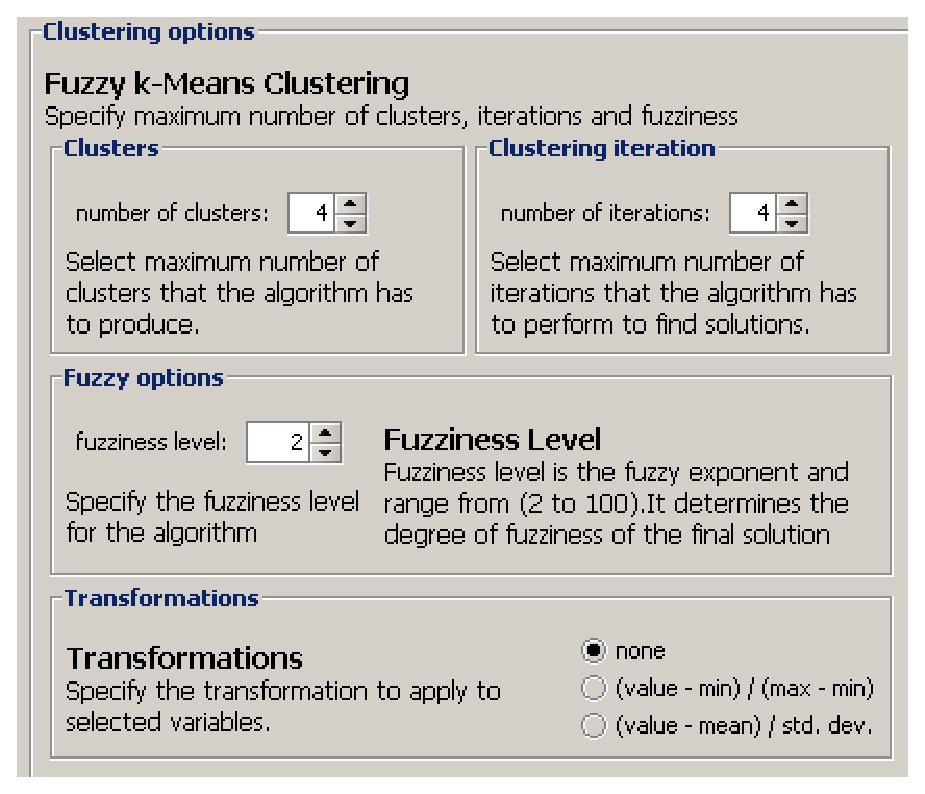
\includegraphics[scale=.5]{img/jwat/Manual/fuzzy_options.eps}
\end{center}
    \caption{Parameters of the clustering algorithm Fuzzy k-Means}
    \label{fig:fuzzy_options}
\end{figure}
\subsection{The results of a clustering execution}
At the end of the execution of a clustering algorithm the tab that
allows the analysis of the results is shown. The main panel shows
the table in \autoref{fig:list_clustering} that contains the
algorithm(s) executed and the maximum number of clusters
identified. It is possible to delete the results of an execution
by clicking the button

\includegraphics[scale=.8]{img/jwat/Manual/del_button.eps}
in the last column.
\begin{figure}[htbp]
\begin{center}
    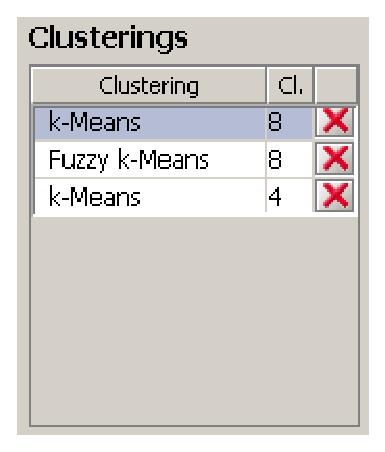
\includegraphics[scale=.5]{img/jwat/Manual/list_clustering.eps}
\end{center}
    \caption{List of executed clustering algorithms }
    \label{fig:list_clustering}
\end{figure}

Depending on the selected clustering algorithm different results
panels are shown in the results table.
\subsubsection{K-Means algorithm results}
\label{cha:usrman:rkmean} When the $k-Means$ algorithm results are
selected, a table reporting the indices concerning the goodness of
the partitions is
shown, \autoref{fig:kmeans_list}.\\
To estimate the optimal number $k$ of clusters in which the given
set of observations will be subdivided two indicators of the
goodness of a partition are used. For each variable the
\emph{Overall Mean Square Ratio, OMSR}, i.e., a measure of the
reduction of within-cluster variance between partitions in $k$ and
in $k+1$ clusters, and the \emph{ratio} of the variance among the
clusters and the within-cluster variance have been used. Large
values of the $OMSR$ justify increasing the number of clusters
from $k$ to $k+1$. An optimal partition should also be
characterized by values greater than 1 of the \emph{ratio}s of the
variances among the clusters and within the clusters for each
variable.

A visual indication of the goodness of a partition is given with
the icons

\includegraphics[scale=.25]{img/jwat/Manual/Measure_ok.eps} and

\includegraphics[scale=.25]{img/jwat/Manual/Measure_fail.eps}
representing good and bad results respectively. The values of OMSR
and of the \emph{ratio} are also reported in the table.

By selecting one of the rows of the table in 
\autoref{fig:kmeans_list} the panel is updated and in the right side a
tabs structure concerning the visualization of the results is
shown. Three main panels are available (\autoref{fig:kmenas_c_info}):
\begin{figure}[htbp]
\begin{center}
    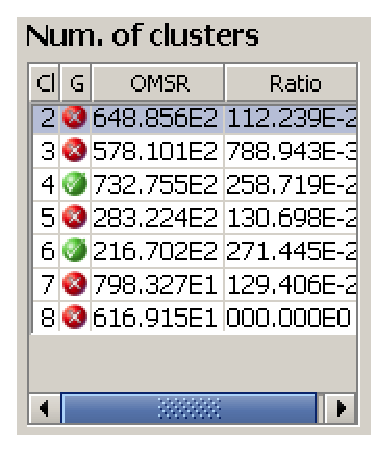
\includegraphics[scale=.5]{img/jwat/Manual/kmeans_list.eps}
\end{center}
    \caption{Indicators of the goodness of a partition
    (\emph{Overall Mean Square Ratio} and \emph{ratio} indices)
    for the K-Means algorithm}
    \label{fig:kmeans_list}
\end{figure}
\begin{itemize}
\item \emph{Clustering Info: }It shows some statistical
information concerning the clusters. For each cluster the number
of its components and its weight with respect to the total
population are reported. Pie-charts are also used to visualize
these data. The panel at the bottom shows for each variable the
distribution (in \%) of its values among the clusters.
\begin{figure}[htbp]
\begin{center}
    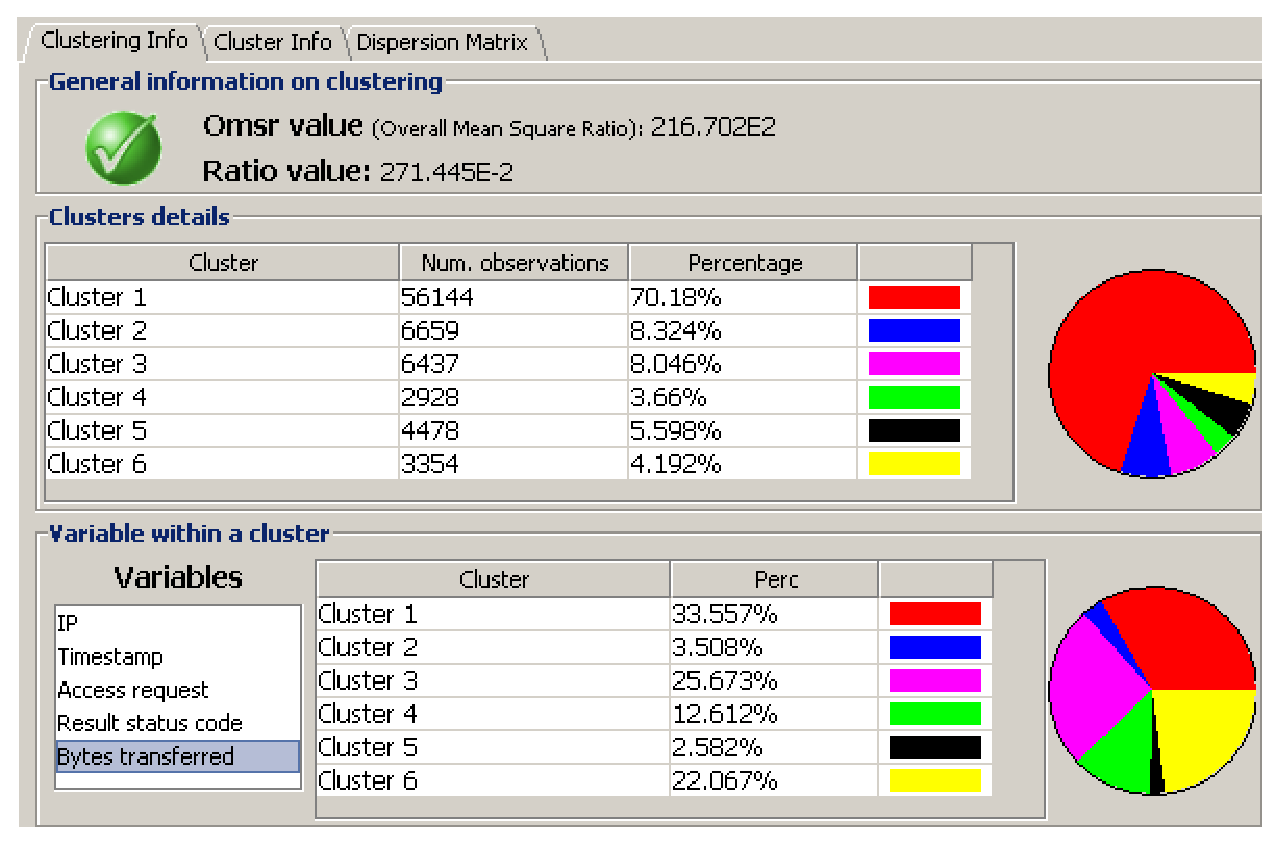
\includegraphics[scale=.5]{img/jwat/Manual/kmenas_c_info.eps}
\end{center}
    \caption{Characterization of the clusters}
    \label{fig:kmenas_c_info}
\end{figure}
\item \emph{Clusters Info: }It shows statistics concerning the
clusters (\autoref{fig:kmeans_cg_info}). Besides the classic
descriptive univariate statistics, the \emph{ISC}, that indicates
which variables have been used for the clustering, and the
\emph{center} values, that refer to the centroid coordinates of
each cluster, are reported. The panel at the bottom shows a
preview (it can be magnified by a left double click of the mouse)
of the graph concerning the comparisons of the distributions of
the variables used in each cluster. It is also possible to
visualize the list of observations that belong to a cluster
through the \emph{`Show Observations'} button (attention! this
operation may requires several minutes).
\begin{figure}[htbp]
\begin{center}
    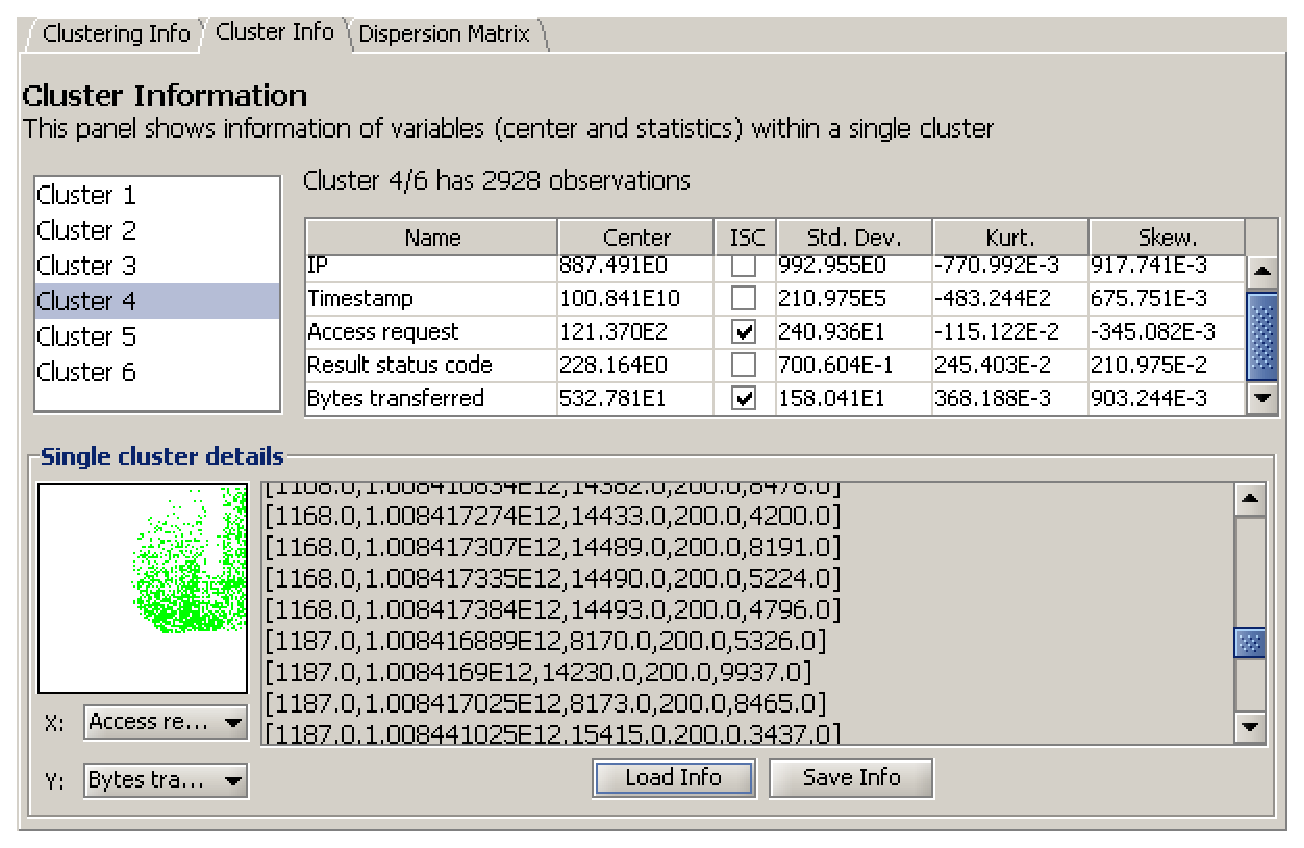
\includegraphics[scale=.5]{img/jwat/Manual/kmeans_cg_info.eps}
\end{center}
    \caption{Descriptive statistics of the clusters obtained with the k-means
    algorithm and their visual
    characterization through the dispersion matrix}
    \label{fig:kmeans_cg_info}
\end{figure}
\item \emph{Dispersion Matrix:} this panel shows the matrix of all
the possible variable \emph{vs} variable scatter plots (\autoref{fig:kmean_8_matrix}). These graphs allows a visual
interpretation of the compositions of the clusters since the
observations are represented with the color corresponding to the
cluster it is assigned. With a left double click of the mouse on a
preview, the graph is magnified and several options can be
selected with a right click on the graph.
\begin{figure}[htbp]
\begin{center}
    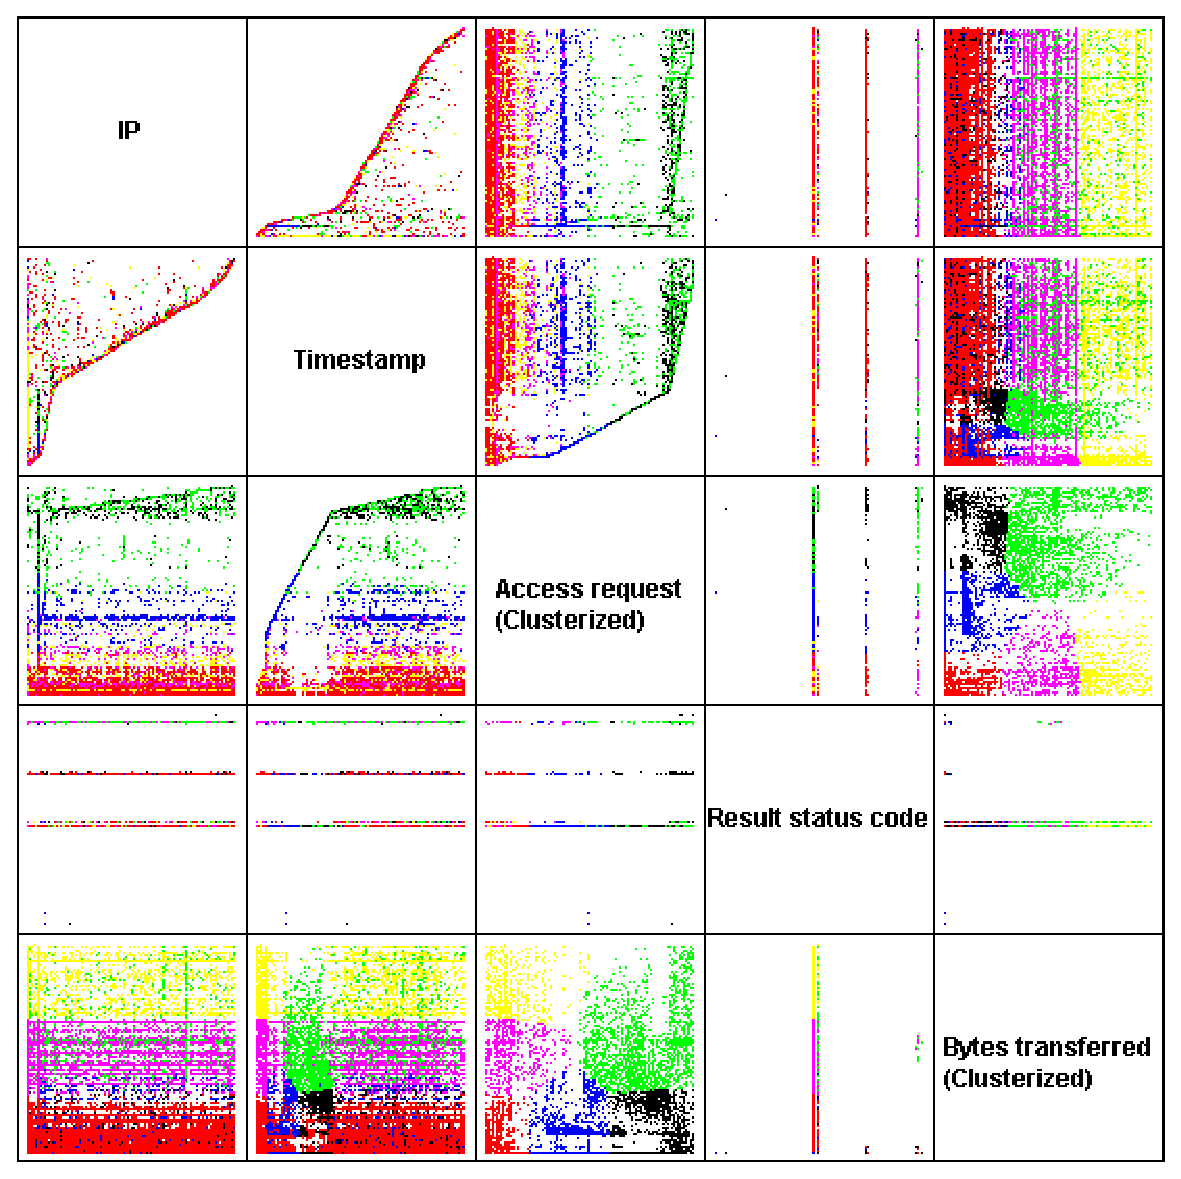
\includegraphics[scale=.5]{img/jwat/Manual/kmean_8_matrix.eps}
\end{center}
    \caption{K-Means scatter plots matrix. Each observation is represented
    with the color corresponding to the cluster it is assigned.}
    \label{fig:kmean_8_matrix}
\end{figure}
\end{itemize}
%\clearpage
\subsubsection{Fuzzy K-Means algorithm results}
\label{cha:usrman:rfuzzy} When the fuzzy k-Means results are
selected, the panel is uploaded and in the table of 
\autoref{fig:list_clustering} a new table containing a row for each
partition identified is shown (\autoref{fig:kmeans_list}). The
number of clusters, the \emph{Entropy} index and the \emph{ratio}
are shown. By selecting one of the rows of table in 
\autoref{fig:fuzzy_list} the panel is updated and appears in the right
side a tabs structure that permits to visualize information
concerning results, by grouping them in three main panels:
\begin{figure}[htbp]
\begin{center}
    \includegraphics[scale=.5]{img/jwat/Manual/fuzzy_list.eps}
\end{center}
    \caption{Results of a fuzzy k-Means algorithm execution}
    \label{fig:fuzzy_list}
\end{figure}
\begin{itemize}
\item \textit{Clustering Info: }It shows the clusters that have
been identified and the entropy values (
\autoref{fig:fuzzy_c_info}). The error value used to identify a
partition should be set by the user and can be easily changed
(error setting information are reported on the right). Pressing
the `\emph{Apply error}' button the assignment of the observations
in the current partitions will be changed according to the new
error value and the table at the bottom showing the composition of
each cluster (and the statistical and graphic information) of the
following panels will be updated. Note that the sum of the
percentages could be \emph{greater} than 100\% because of the
multiple assignments of the fuzzy algorithm.
\begin{figure}[htbp]
\begin{center}
    \includegraphics[scale=.5]{img/jwat/Manual/fuzzy_c_info.eps}
\end{center}
    \caption{Results of a fuzzy k-means algorithm execution}
    \label{fig:fuzzy_c_info}
\end{figure}
\item \textit{Clusters Info: }It shows statistical information
concerning the selected cluster (\autoref{fig:fuzzy_cg_info}).
See the comments reported above for the cluster info of the
k-means algorithm.
\begin{figure}[htbp]
\begin{center}
    \includegraphics[scale=.5]{img/jwat/Manual/fuzzy_cg_info.eps}
\end{center}
    \caption{Descriptive statistics of the clusters obtained with the fuzzy
    k-means algorithm and their visual
    characterization through the dispersion matrix}
    \label{fig:fuzzy_cg_info}
\end{figure}
\item \textit{Dispersion Matrix: }this last panel shows the matrix
of all the possible variable vs. variable scatter plots (
\autoref{fig:fuzzy_4_matrix}). See the comments reported above for the
dispersion matrix of the k-means algorithm.
\begin{figure}[htbp]
\begin{center}
    \includegraphics[scale=.5]{img/jwat/Manual/fuzzy_4_matrix.eps}
\end{center}
    \caption{Fuzzy k-Means scatter plot matrix. Each observation is represented
    with the color corresponding to the cluster it is assigned}
    \label{fig:fuzzy_4_matrix}
\end{figure}
\end{itemize}
\clearpage

\subsection{An example of a web log analysis}
In this section we will describe an example of application of the
JWAT tool for a workload analysis. The analyzed set of data
consists of observations stored in the log file of a web server
of a university site.\\
The input file \emph{Demo1Data.jwat} and its format
\emph{Demo1Format.jwatformat} can be found in the subfolders
\textit{Examples} and \textit{jwatFormats}, respectively, of the
Java Modelling Tools folder installed with the JMT tools.\\

\textbf{Step 1 - Input panel}\\
\begin{figure}[htbp]
        \begin{center}
            \includegraphics[scale=.5]{img/jwat/Examples/rows_example.eps}
        \end{center}
        \label{fig:rows_example}
        \caption{Example of observations in the input file considered.}
\end{figure}
\begin{figure}[htbp]
        \begin{center}
            \includegraphics[scale=.5]{img/jwat/Examples/WebLogfmt.eps}
        \end{center}
        \caption{Input format example}
        \label{fig:rows_example1wa}
\end{figure}

Each observation consists of the values of 4 variables described
in \autoref{fig:rows_example1wa}:
\begin{itemize}
    \item \textit{IP}: String type variable that defines IP address of the request.
    \item \textit{Timestamp}: Date type variable that defines the timestamp of the request,
    the regular expression\begin{verbatim}"\d\d/\w\w\w/\d\d\d\d:\d\d:\d\d:\d\d"' \end{verbatim}
    identifies that the data will be in the format dd/mmm/yyyy:hh:mm:ss (e.g., 12/Jun/2000:12:21:45).
    \item \textit{Access request}: String type variable that identifies the object that is
    the target
    of the request. The definition through delimiter " and regular expression "`.*"'
    allows the reading of all the string that is contained between
    quotation marks;
    if it is necessary it is
    possible to modify the expression "`.*"' to read only a part of the string between
    quotation marks.
    \item \textit{Bytes transferred}: Numeric type variable that identifies the quantity
    of bytes transferred due to the execution of the request submitted.
\end{itemize}

\textbf{Step 2 - Descriptive statistics and sample extraction}\\
Before the execution of the cluster analysis the size of the input
data set has been reduced executing the filter \emph{Interval} to
the values of the variable \emph{Bytes transferred} setting a
maximum value of 20000 and a minimum value of 0. The purpose of
this filtering operation is to obtain a data set more compact but
still representative of the original one. In Tables
\autoref{descr_stat_before} and \autoref{descr_stat_after} the descriptive
statistics before and after applying the filter on the input data
are shown, respectively. Scatter plot matrix of the filtered data
are shown in \autoref{scatters_of_ex1_ after}.
\begin{figure}[htbp]
        \begin{center}
            \includegraphics[scale=.5]{img/jwat/Examples/stats_prima.eps}
        \end{center}
        \caption{Descriptive statistics of the original data before
        applying the filter on the "Bytes transferred" variable}
        \label{descr_stat_before}
\end{figure}
\begin{figure}[htbp]
        \begin{center}
            \includegraphics[scale=.5]{img/jwat/Examples/stats_dopo.eps}
        \end{center}
        \caption{Descriptive statistics of the original data after
        applying the filter on the "Bytes transferred" variable}
        \label{descr_stat_after}
\end{figure}
\begin{figure}[htbp]
        \begin{center}
            \includegraphics[scale=.4]{img/jwat/Examples/scatter_matrix.eps}
        \end{center}
        \caption{Scatters matrix on the data set after applying the
        filter on the "Bytes transferred" variable.}
        \label{scatters_of_ex1_ after}
\end{figure}
\\ About 2500 observations have been dropped due to the filtering action,
reducing considerably the variance.\\

\textbf{Step 3 - Clustering panel}\\
The k-Means algorithm and the variables \emph{timestamp} and
\emph{Bytes transferred} have been selected in the clustering
panel together with the following options: number of clusters 7,
interactions 50 and transformation \emph{Max-Min}. The clustering
results panel is opened automatically. Through the \emph{`Back'}
button we went back to the previous panel to execute a new
clustering algorithm. The fuzzy k-Means algorithm and the
variables \emph{timestamp} and \emph{Bytes transferred} have been
selected together with the following options: number of clusters
6, interactions 20, fuzziness level 2.0.\\


\textbf{Step 4 - Results panel}\\
The results concerning the goodness of the partitions obtained
with the two clustering algorithms are reported in the following
tables:
\begin{multicols}{3}
        \begin{center}
        \includegraphics[scale=.5]{img/jwat/Examples/list_clustering.eps}\\
        Clustering algorithms
        \end{center}
        \columnbreak
        \begin{center}
        \includegraphics[scale=.5]{img/jwat/Examples/list_kmenas_clustering.eps}\\
        k-Means
        \end{center}
        \columnbreak
        \begin{center}
        \includegraphics[scale=.5]{img/jwat/Examples/list_fuzzy_clusters.eps}\\
        Fuzzy k-Means
\label{global_results}
        \end{center}
        \columnbreak
\end{multicols}
We have visualized different statistics for each algorithm by
varying the number of clusters, in particular we show the scatter
plots matrix for the partition with 5 clusters (as can be seen
from the OMSR values this partition has been evaluated as a good
one).
\begin{figure}[htbp]
        \begin{center}
            \includegraphics[scale=.5]{img/jwat/Examples/matrix_kmeans.eps}
        \end{center}
        \caption{K-Means algorithm scatter plots matrix}
\end{figure}
\begin{figure}[htbp]
        \begin{center}
            \includegraphics[scale=.5]{img/jwat/Examples/matrix_fuzzy.eps}
        \end{center}
        \caption{Fuzzy k-Means algorithm scatter plots matrix}
\end{figure}
\clearpage

\subsection{Menus description}
\label{sec:usrman:desc_menu}
\subsubsection{File}
\textbf{New} Use this command to start a new analysis selecting a
new log file.

\noindent
\begin{tabular}{ll}
Shortcut on Toolbar: & \includegraphics[scale=.8]{img/jwat/Manual/new.eps}\\
Accelerator Key: & CTRL+N
\end{tabular}

\subsubsection{Exit}
Use this command to terminate the JWAT current session. It is
possible to utilize `\emph{Exit}' button in the buttons bar of
application. If the session has been modified after its creation
or after its last saving, a popup window asks confirmation to save
session.

\noindent
\begin{tabular}{ll}
\\
Accelerator Key: & CTRL+Q
\end{tabular}

\subsubsection{Action}
\textbf{Solve} Use this command, when enabled, to start the
algorithm selected in the clustering panel. It is possible to
obtain the same result by using `\emph{Solve}' button in the
buttons bar of the application.

\noindent
\begin{tabular}{ll}
Shortcut on Toolbar: & \includegraphics[scale=.8]{img/jwat/Manual/sim.eps}\\
Accelerator Key: & CTRL+L
\end{tabular}

\subsubsection{Help}
\textbf{JWAT Help} Use this command to visualize the help.
Suggestions concerning the single tab in the application are also
available by using the `\emph{Help}' button in the buttons bar of
application.

\noindent
\begin{tabular}{ll}
Shortcut on Toolbar: & \includegraphics[scale=.8]{img/jwat/Manual/help.eps}\\
Accelerator Key: & CTRL+Q
\end{tabular}

\subsubsection{About}
Use this command to visualize information concerning JWAT
application.

\clearpage
\section{Format definition}
\label{sec:usrman:es_def_form} In this section we will describe
the format definition of the file in input to the application. We
will introduce the basic concepts on which the format specific is
based and then we will describe some examples with different
files.

The application allows, by using regular expression, to utilize as
input either log files of standard formats, as Apache and IIS, or
log files modified by the user. The only important requirement on
the input file structure is that every observation (i.e., the set
of the variables that refer to one element/item considered) must
end with `$\backslash$n' character (new line).

To allow the application to be able to process correctly a log
file, the user must describe:
\begin{itemize}
\item the observation structure, that is the number of variables
that compose it. \item and for each variable the name, the type
and the `structure'.
\end{itemize}
These information are specified by the user through the input
panel described in Section~\ref{sec:usrman:sel_def_format}.

Regarding the number of variables it is enough to insert in the
format table a number of rows equal to the number of elements that
compose the observation (see Section~\ref{sec:usrman:sel_def_format:man}). In \autoref{fig:add_vars}
the observation is composed of 6 variables.
\begin{figure}[htbp]
\begin{center}
    \includegraphics[scale=.5]{img/jwat/Format/add_vars.eps}
\end{center}
    \caption{Format table after the insertion of the number of variables}
    \label{fig:add_vars}
\end{figure}

The definition of the single variable requires, in addition to the
name, a comment, its selection in order to be considered in the
analysis or not, its type, the description of the possible
delimiter (Separator) and of the regular expression that
characterizes it.

The type has to be chosen among the \emph{numeric, string o data}.
The delimiter defines (if it exists) the character or the
characters that delimit the variable's value. The regular
expression (Perl 5) defines the format with which the variable
value is recorded in the log file.

A concise description of the format used for the regular
expressions (Perl 5) follows. The purpose of the definition of the
regular expression is to specify the pattern that the variable
values must have and therefore (together with selected type) to
allow the application to process correctly its value. For a
complete description of the regular expressions see a Mastering
regular expressions book. In this section we will describe some
options useful to define in a simple way the pattern of the
variables values. A list of operators follows:
\begin{description}\addtolength{\itemsep}{-0.3\baselineskip}
\item [+]: it indicates that there are one or more instances of
the preceding character ( a+ $\Rightarrow$ a,aa,aaa,...) \item
[[]]: it defines a pattern that allows to utilize as match element
one of the values within square brackets ( a[bcd]e $\Rightarrow$
abe, ace, ade) \item [*]: it indicates that there are zero or more
instances of the preceding character ( ba* $\Rightarrow$
b,ba,baa,baaa,...) \item [?]: it indicates that there are zero or
one instance of the preceding character ( ba? $\Rightarrow$ b,ba)
\item [\textasciicircum]: it has two different meanings depending
on the use. The former permits to require that a pattern starts
with a particular character (\textasciicircum abc $\Rightarrow$
abcdef,abc fg,...). If it is utilized within square brackets as
first character, it allows to match any character that doesn't
belong to the defined group ([\textasciicircum a] $\Rightarrow$
bcd,wedfgr,...) \item [()]: it defines a pattern that permits to
use as match element the string that is contained between brackets
((ab)+ $\Rightarrow$ ab,abab,ababab,...).
\end{description}
A list of \emph{Escape Sequences } used to identify intervals of
characters follows:
\begin{description}\addtolength{\itemsep}{-0.3\baselineskip}
\item [$\backslash$d]: it identifies whichever number [0-9]. \item
[$\backslash$D]: it identifies whichever thing except a number
[\textasciicircum 0-9]. \item [$\backslash$w]: it identifies
whichever character or number [0-9a-zA-Z]. \item [$\backslash$W]:
it identifies whichever thing except a character or a number
[\textasciicircum 0-9a-zA-Z]. \item [$\backslash$s]: it identifies
 a \emph{white space} character
[$\backslash$t$\backslash$n$\backslash$r$\backslash$f]. \item
[$\backslash$S]: it identifies whichever thing except a
\emph{white space} character [\textasciicircum
$\backslash$t$\backslash$n$\backslash$r$\backslash$f]. \item [.]:
it identifies whichever character except the \emph{new line}
character `$\backslash$n'.
\end{description}
Combining in an opportune way the characters, the options and the
\emph{Escape Sequences }it is possible to define correctly the
regular expression for each variable.

In the specific of regular expressions in Perl 5 there are some
characters that are considered \emph{metacharacters}. Some of them
are the same operators defined before. In this case, to use such
characters as elements in the expression is enough to precede them
with the $\backslash$ character.

The delimiter identifies one or more characters that delimit the
value of a variable. In the log file of the Apache format the page
URL requested by the user contains characters and spaces and is
delimited by ``''. A simple definition of the
\emph{$\backslash$w+} type regular expression could produce a
wrong result because the value recovered by application would
finish at the first met space and not at the closure ''. To avoid
this problem it is possible to utilize the delimiters so that by
using the expression \emph{.+} and specifying as delimiter '' the
result will be correct.

Concerning the Apache log file, and more precisely the
\emph{timestamp} field, it is possible to show another use of the
delimiter. The value is contained between characters `[' e `]'
(e.g, \emph{[12/Dec/2001:00:00:03 +0100]}) and by using the field
delimiter it is possible to specify as regular expression the
following:
\begin{center}
$\backslash$d$\backslash$d/$\backslash$w$\backslash$w$\backslash$w/
$\backslash$d$\backslash$d$\backslash$d$\backslash$d:$\backslash$d$
\backslash$d:$\backslash$d$\backslash$d:$\backslash$d$\backslash$d
\end{center}
This expression doesn't specify the last part of the field
(\emph{+0100}) but it is correct in any case because specifying
the delimiters it is possible to define the regular expression in
order to match only a part of the variable value.

\subsection{Example of a format definition}
Let's consider a file to be analyzed with the following structure
of the observations:
\begin{center}
\emph{\footnotesize String without spaces 1000 0.0876 -12.663
``String with spaces'' [12/Dec/2001:00:00:03 +0100]}
\end{center}
The variables are 6 and their definition (
\autoref{fig:format_1}) is the following:
\begin{description}
\item [String without spaces :]we can define the regular
expression in different ways, as for example \emph{[a-zA-Z]+} if
the string doesn't contain numbers or \emph{$\backslash$w+} to
indicate whichever string of numbers and characters. \item
[Integer number :] we define the regular expression as a sequence
of one or more numbers and therefore as \emph{$\backslash$d+}.
\item [Positive decimal :] in this case there is the possibility
to have decimal digits so that we define the regular expression as
a sequence of one or more digits (\emph{$\backslash$d+}) that may
have the decimal separator and a further succession of one or more
digits. The result is therefore
\emph{$\backslash$d+([$\backslash$.]$\backslash$d+)?}. \item
[Decimal with sign :] in this case in comparison to the previous
case there is the possibility that at the beginning of the number
there is a sign +, - or no sign. Therefore it is enough to add at
the beginning of the regular expression \emph{([+-])?}. \item
[String with spaces :] if we utilize the regular expression
previously defined \emph{$\backslash$w+} we would have a problem
because the value recovered from the log file would be ''String
that is not correct. The best solution is to utilize the
delimiter, in this case \emph{''}, and to utilize therefore the
definition \emph{.+}. \item [Date :] even in this case by using
the delimiter (\emph{[]}) we can define the following regular
expression
$\backslash$d$\backslash$d/$\backslash$w$\backslash$w$\backslash$w/
$\backslash$d$\backslash$d$\backslash$d$\backslash$d:$\backslash$d
$\backslash$d:$\backslash$d$\backslash$d:$\backslash$d$\backslash$d
that may be used to recover the only information
``12/Dec/2001:00:00:03'' leaving out the remaining part.
\end{description}
\begin{figure}[htbp]
\begin{center}
    \includegraphics[scale=.5]{img/jwat/Format/formato_1.eps}
\end{center}
    \caption{Example of the definition of a file format}
    \label{fig:format_1}
\end{figure}
\subsection{Example of the definition of the Apache log}
Now we will describe the format of the Apache log. Each
observation has the following structure:
\begin{center}
\emph{\footnotesize 151.29.12.105 - - [12/Dec/2001:00:00:10 +0100]
``GET /mappe HTTP/1.1'' 200 313 www.polimi.it
``http://www.polimi.it/'' ``Mozilla/4.0 (compatible; MSIE 5.0;
Windows 98; DigExt)'' ``-''}
\end{center}
A brief explanation of the regular expressions used (\autoref{fig:format_2}) follows:
\begin{enumerate}
\item for the Ip address of the request we define a sequence of
one or more digits separated by a point and therefore the regular
expression is
\emph{$\backslash$d+$\backslash$.$\backslash$d+$\backslash$.$\backslash$d+$\backslash$.
$\backslash$d+}. \item in most cases no value is set, and
therefore it is possible to define exactly the string that we want
to recover from the file through \emph{- -} (it is advisable not
to select this variable at the moment of loading). \item for the
date we use the same definition described in the previous example
or more simply by selecting the date type in the concerning box,
the application supplies a default definition that is correct too.
\item it is a string, delimited by '', that can contains within
some spaces characters and numbers. The best definition uses the
delimiter and the regular expression \emph{.+}. \item it is an
integer number and as we have seen before we can utilize a more
simple regular expression \emph{$\backslash$d+} o
\emph{([+-])?$\backslash$d+([$\backslash$.] $\backslash$d+)?}.
\item even in this case it is an integer number and as we have
seen before we can utilize the regular expression
\emph{$\backslash$d+} o
\emph{([+-])?$\backslash$d+([$\backslash$.] $\backslash$d+)?}.
\item in this case the string is not delimited by any particular
character and it doesn't contain any spaces so that we can utilize
a simple regular expression \emph{$\backslash$w+} or ones little
bit different as \emph{[\textasciicircum$\backslash$s]+}. \item
these last three strings are all delimited by the character '' and
they can contain some spaces, characters or numbers and therefore
we must utilize the regular expression \emph{.+}.
\end{enumerate}
\begin{figure}[htbp]
\begin{center}
    \includegraphics[scale=.5]{img/jwat/Format/formato_2.eps}
\end{center}
    \caption{Apache log file format definition}
    \label{fig:format_2}
\end{figure}
